\chapter{Chapter 2 appendix}
\section{Packed cell volume is an overestimate in common cancer cell lines}
\label{app_ch2_cell_vol}
This is an abridged version of the method and results in Engstrom et al. 2021 \cite{Engstrom2021-az}.

Originally developed to determine the volume of red cells in blood, or hematocrit, packed cell volume (PCV) measurements have more recently also been used to determine the volume of adherent cell lines for conversion of intracellular metabolite quantities into concentrations \cite{Park2016-ap, Liu2018-it, Yang2020-fs, Ghergurovich2020-nb}.
Another way of determining cell volume is using the Coulter principle which relates particle volume to the change in electrical impedance as the particle passes through an aperture.
For blood, PCV is a reliable measurement, proportional to the cell volume determined using the Coulter principle \cite{Carter1968-xy, Bull2001-xb}; however, this assumption has not been tested for the diverse set of cell lines used for cell culturing.

We compared PCV with Coulter counter-based cell volume measurements for five cell lines and found that the spin protocol provided by the PCV tube manufacturer (2,500 g for 1 min) lead to an overestimate of cell volume compared to Coulter-based measurements.
We hypothesized that this discrepancy is related to incomplete cell packing and that packing efficiency is negatively impacted by ``sticky'' extracellular matrix proteins found abundantly on adherent cells.
This was tested with five different cell lines by increasing the centrifugation speed and time (figure \ref{fig:app_ch2:CCvsPCV}).
The results showed that PCV measurements at the lowest centrifugation speed were overestimates of cell volume compared to Coulter-based measurements for all cell lines.
Adherent cells had the largest volume discrepancy.
PCV measurements decreased with increasing centrifugation speed and time and approached the Coulter-based volume.

In summary, the results indicate that PCV consistently overestimates cell volume compared to measurements using a Coulter counter.
This overestimate in PCV is likely due to incomplete packing, which is particularly problematic for adherent cell lines.
Therefore, it is advisable for future studies relying on accurate cell volume measurements to use the Coulter principle for cell volume measurement.

\begin{figure}[ht]
    \centering
    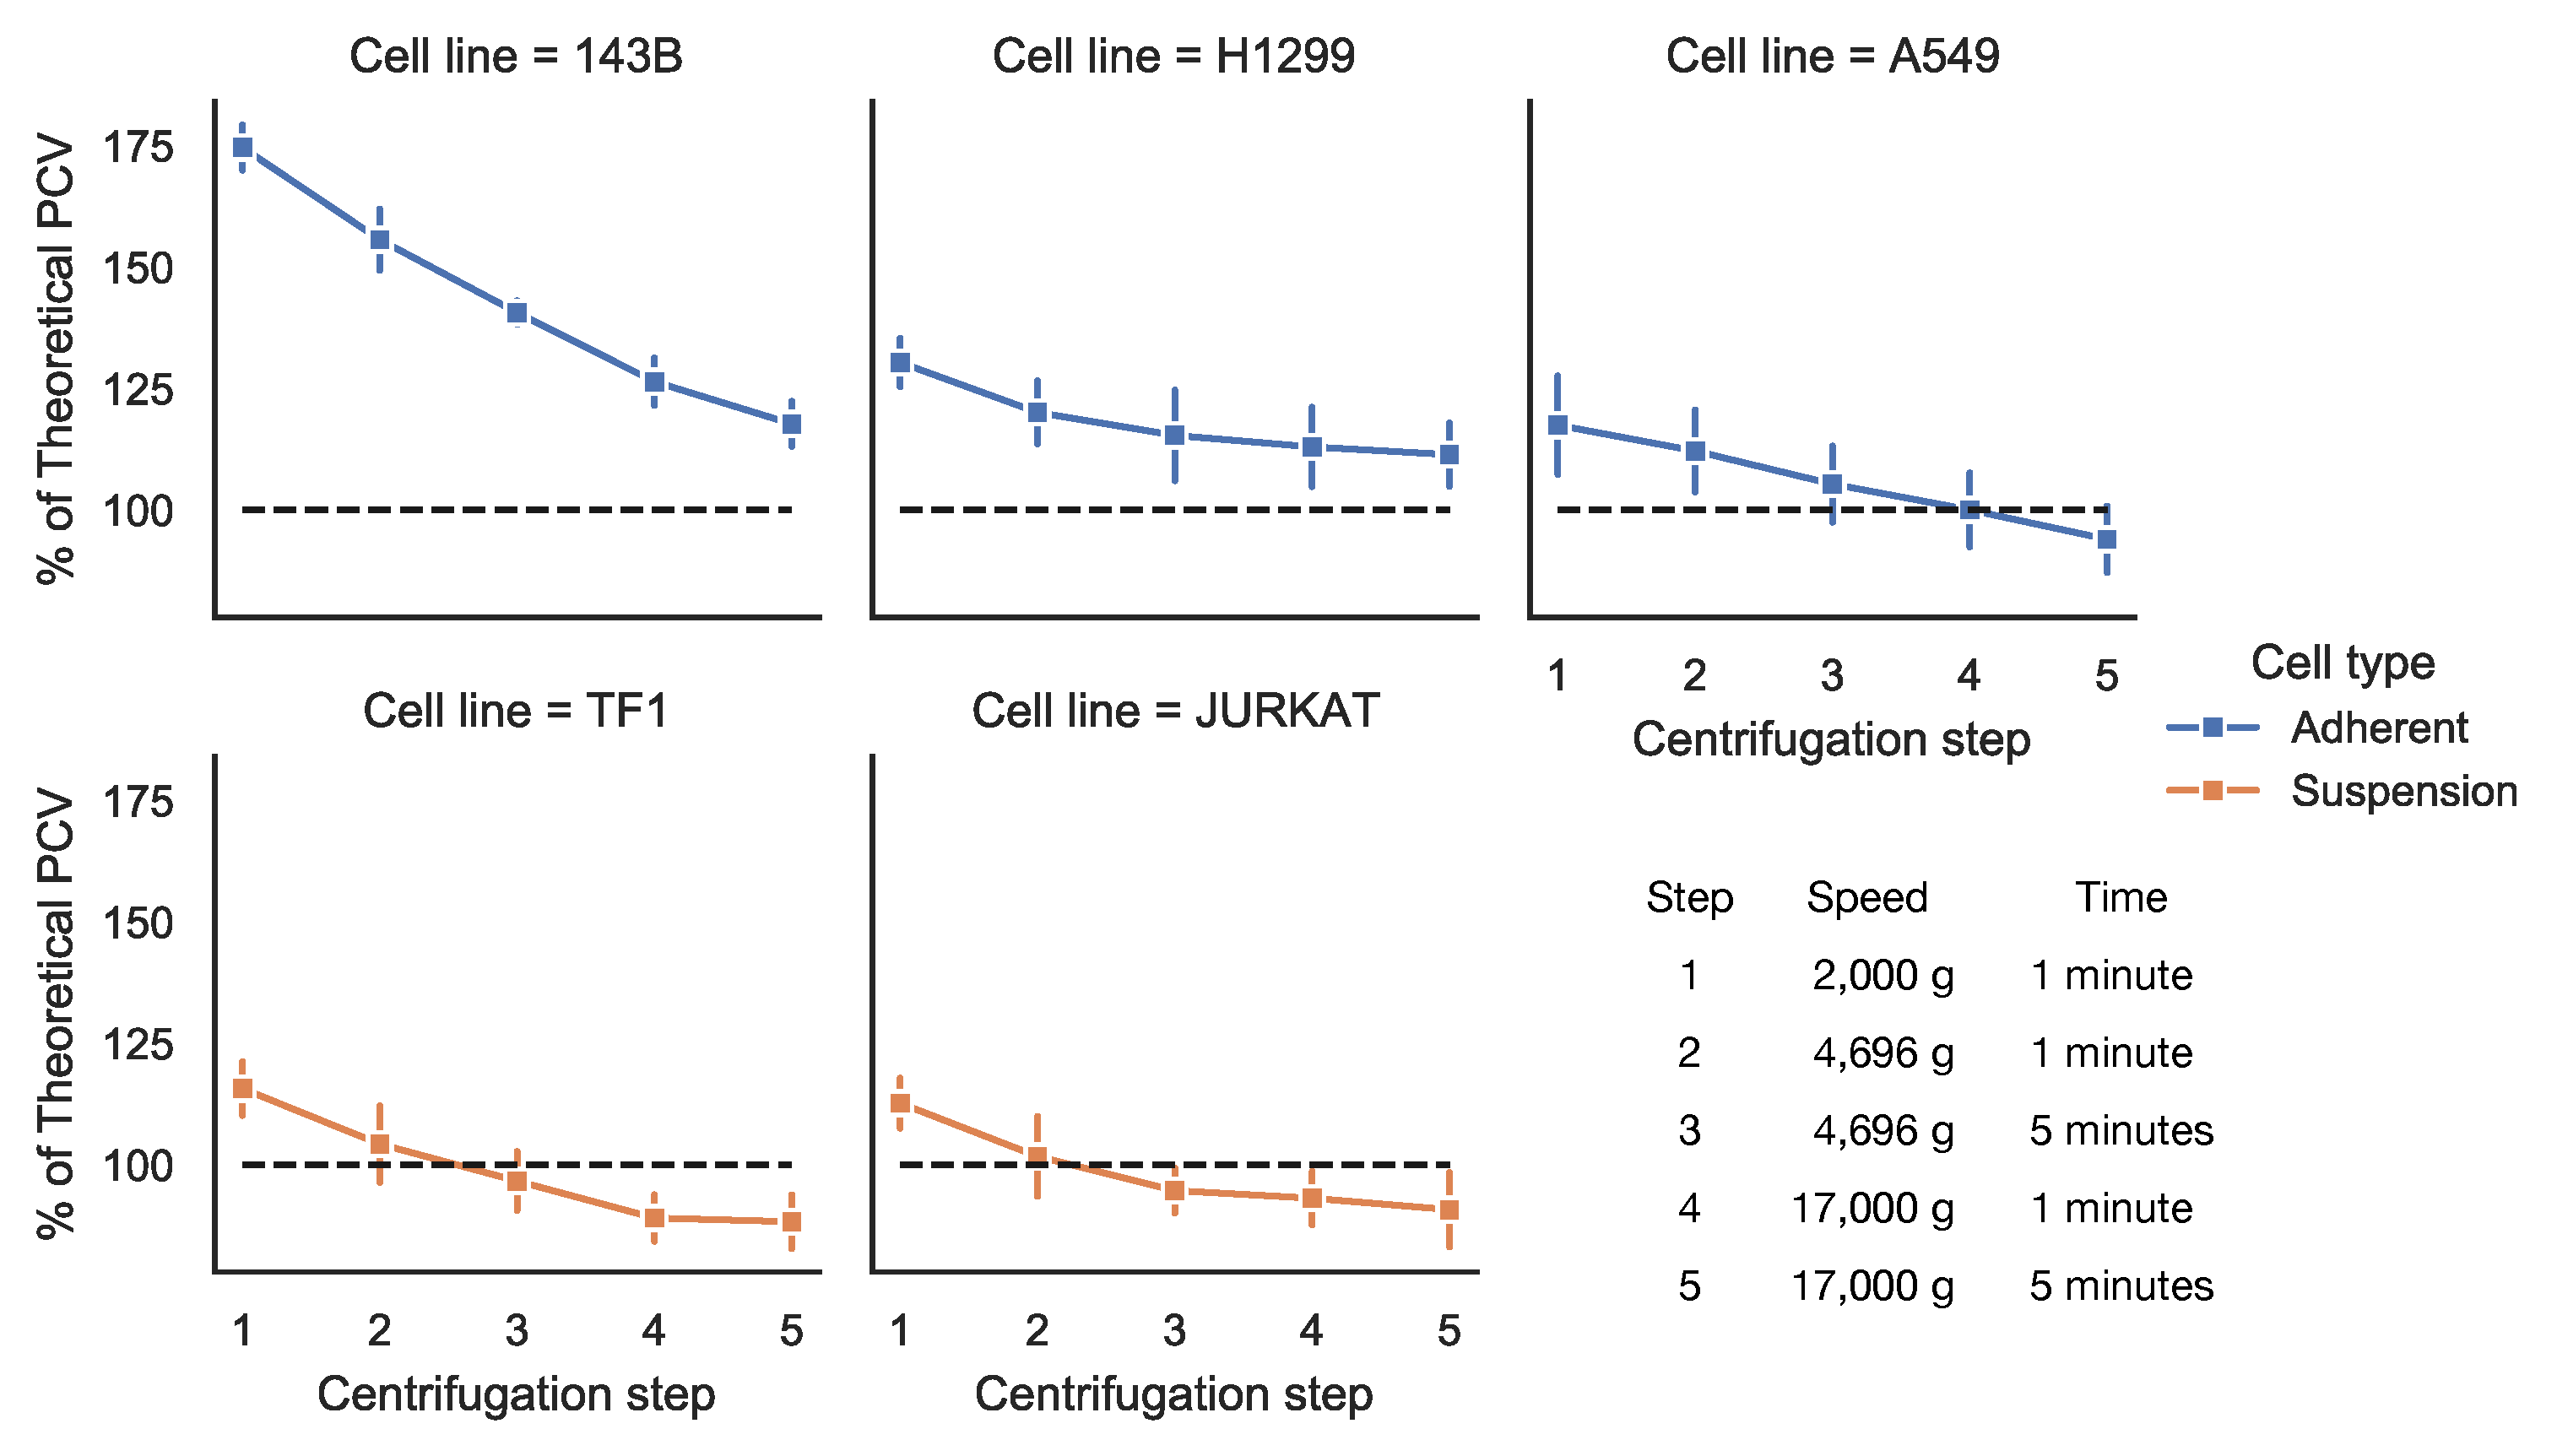
\includegraphics[width=0.99\textwidth]{figures/chap2/app/CCvsPCV.pdf}
    \caption[Packed cell volume vs. Coulter counter]{
    Packed cell volume (PCV) compared to the theoretical volume as determined by a Coulter counter (Multisizer 4).
    }
    \label{fig:app_ch2:CCvsPCV}
\end{figure}




\newpage
\section{Mitochondrial inhibition induces a titratable aspartate limitation}
\begin{figure}[ht]
    \centering
    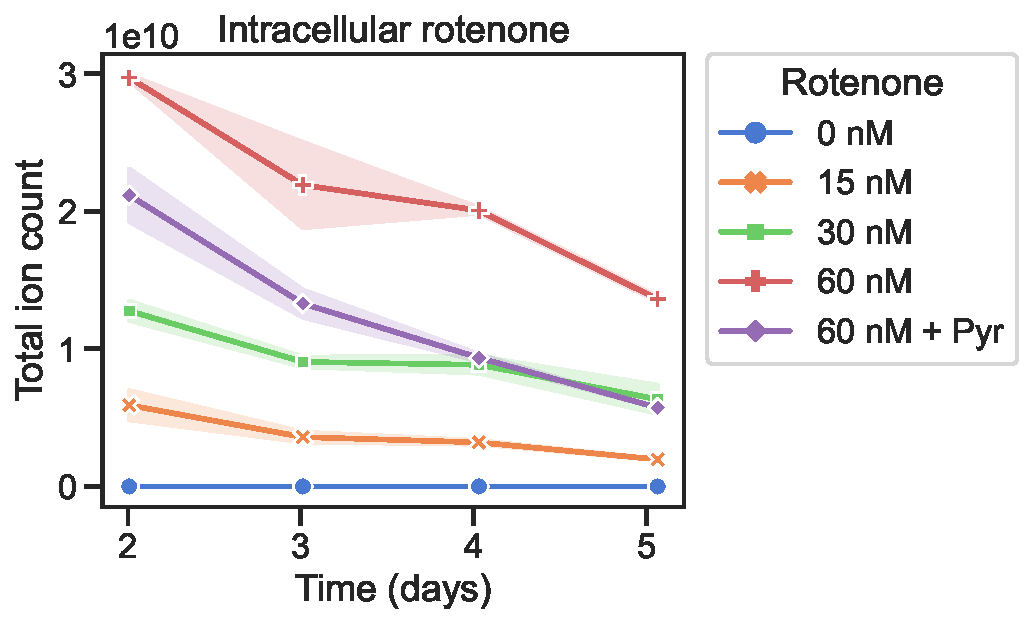
\includegraphics[width=0.45\textwidth]{figures/chap2/app/intra-rotenone-time_rep1.pdf}
    \caption[Rotenone concentration over time.]{
    Rotenone in cell metabolite extract decrease over time after initial treatment indicating degradation.
    Rotenone is known to be degraded in aqueous solutions \cite{Rohan2015-co}.
    Measured as total ion counts using LCMS.
    Related to figure \ref{fig:ch2:NAD_Asp_time}.
    }
    \label{fig:ch2:app:Rot_by_day}
\end{figure}

\begin{figure}[ht]
    \centering
    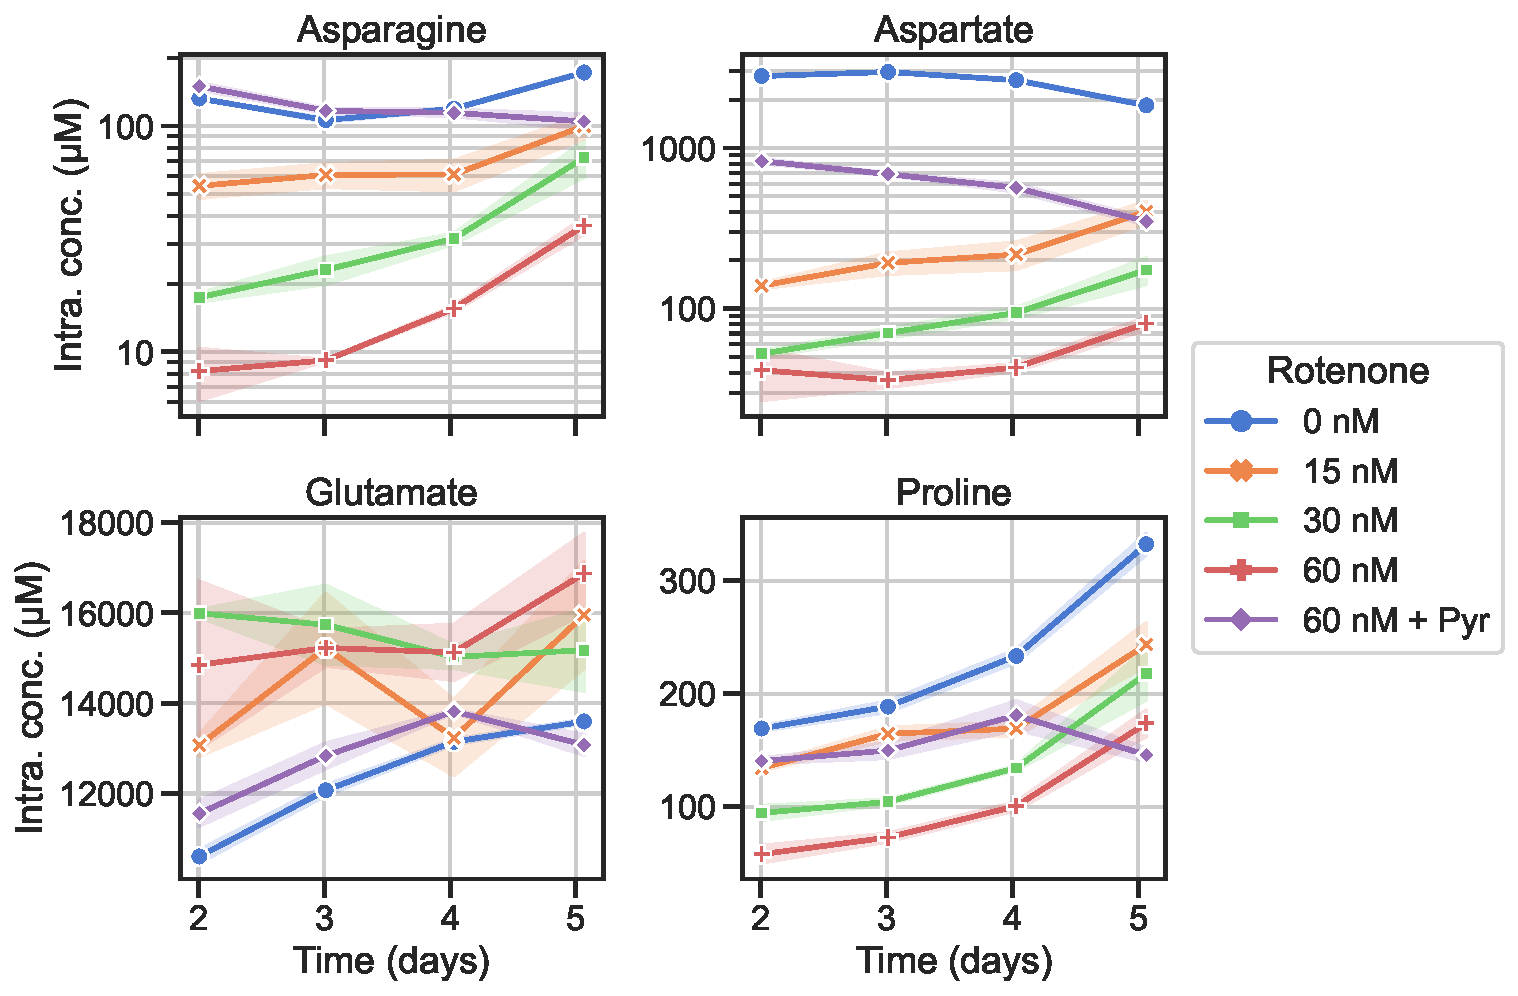
\includegraphics[width=0.8\textwidth]{figures/chap2/app/Asn-Asp-Glu-Pro-time_rep1.pdf}
    \caption[Redox metabolite over time after rotenone.]{
    Intracellular concentration of redox sensitive metabolites over the time course of rotenone treatment.
    Related to figure \ref{fig:ch2:NAD_Asp_time}.
    }
    \label{fig:ch2:app:Metab_by_day}
\end{figure}




%\newpage
\section{Nucleoside, nucleobase and amino acid quantification after acid hydrolysis}
\label{sec:ch2:app:quant}
To quantify cellular nucleotide and amino acid abundance, acid hydrolysis was performed directly on cell material.
Since the hydrolysis was performed in regular plastic tubes with ambient air headspace, there is a risk of oxidation and thus underestimation of the true quantities.
Therefore, amino acid and nucleobase stability was tested in 6 M HCl with 24 hours incubation at 100°C (figures \ref{fig:app_ch2:nucleobase_hydrolysis_stability} and \ref{fig:app_ch2:AA_acid_hydrolysis_stability}).
Samples were prepared with 500 µM amino acid or nucleobase mix and in parallel added either water (MQ) or 6 M HCl.
Water samples were set aside at -20°C.
Amino acids and nucleobases were then quantified using LCMS and each ion count were normalized to its internal standard yielding a response ratio (RR).
For nucleobases, pyrimidines are stable while purines are prone hydrolysis as has been noted previously \cite{Strecker1861-mh, Wulff1892-og, Hunter1936-iu, Markham1949-qy}.
For amino acids, asparagine and glutamine are fully deaminated to produce exactly one equivalent of aspartate and glutamate, respectively.
Tryptophan also breaks down completely while methionine and cystine are broken down but still remain detectable.
Note that histidine is missing due to poor chromatographic separation.  
Thus, acid hydrolysis is compatible with quantification of all pyrimidine nucleobases and all amino acids except asparagine, glutamine, tryptophan, methionine, cystine/cysteine and histidine.

Another potential concern for quantification is low solubility; particularly, of the nucleobases liberated during hydrolysis.
Should any compound hit its solubility limit during processing it would precipitate and its true quantity would be underestimated.
To test the bounds of solubility, increasing amounts of cell material was hydrolyzed in 6 M HCl with 24 hours incubation at 100°C.
Compounds reaching their solubility limit would be expected to show no increase in peak area with increasing amounts of cell material.
This was tested using cell material from a confluent 10 cm dish of 143B cells.
Samples were prepared with 30, 5, 1, 0.2 and 0.05\% of this material, following hydrolysis, drying and reconstitution with 100 µL 80\% LCMS grade methanol.
The resulting quantification (figure \ref{fig:app_ch2:hydrolysis_saturation}) shows that none of the measured nucleosides, nucleobases or amino acids reach their solubility limit.
However, it does display abundant ion suppression which can be corrected by normalization to an internal standard (figure \ref{fig:app_ch2:hydrolysis_AA_saturation_RR}).

The final quantification relies on a calibration curve to convert the internal standard normalized ion count, known as the response ratio, to a concentration.
These curves were fitted for all nucleosides, nucleobases and amino acids that had internal standards and show excellent curve fit, generally spanning concentrations of three orders of magnitude (figure \ref{fig:app_ch2:calibration_curve}).

\begin{figure}[ht]
    \centering
    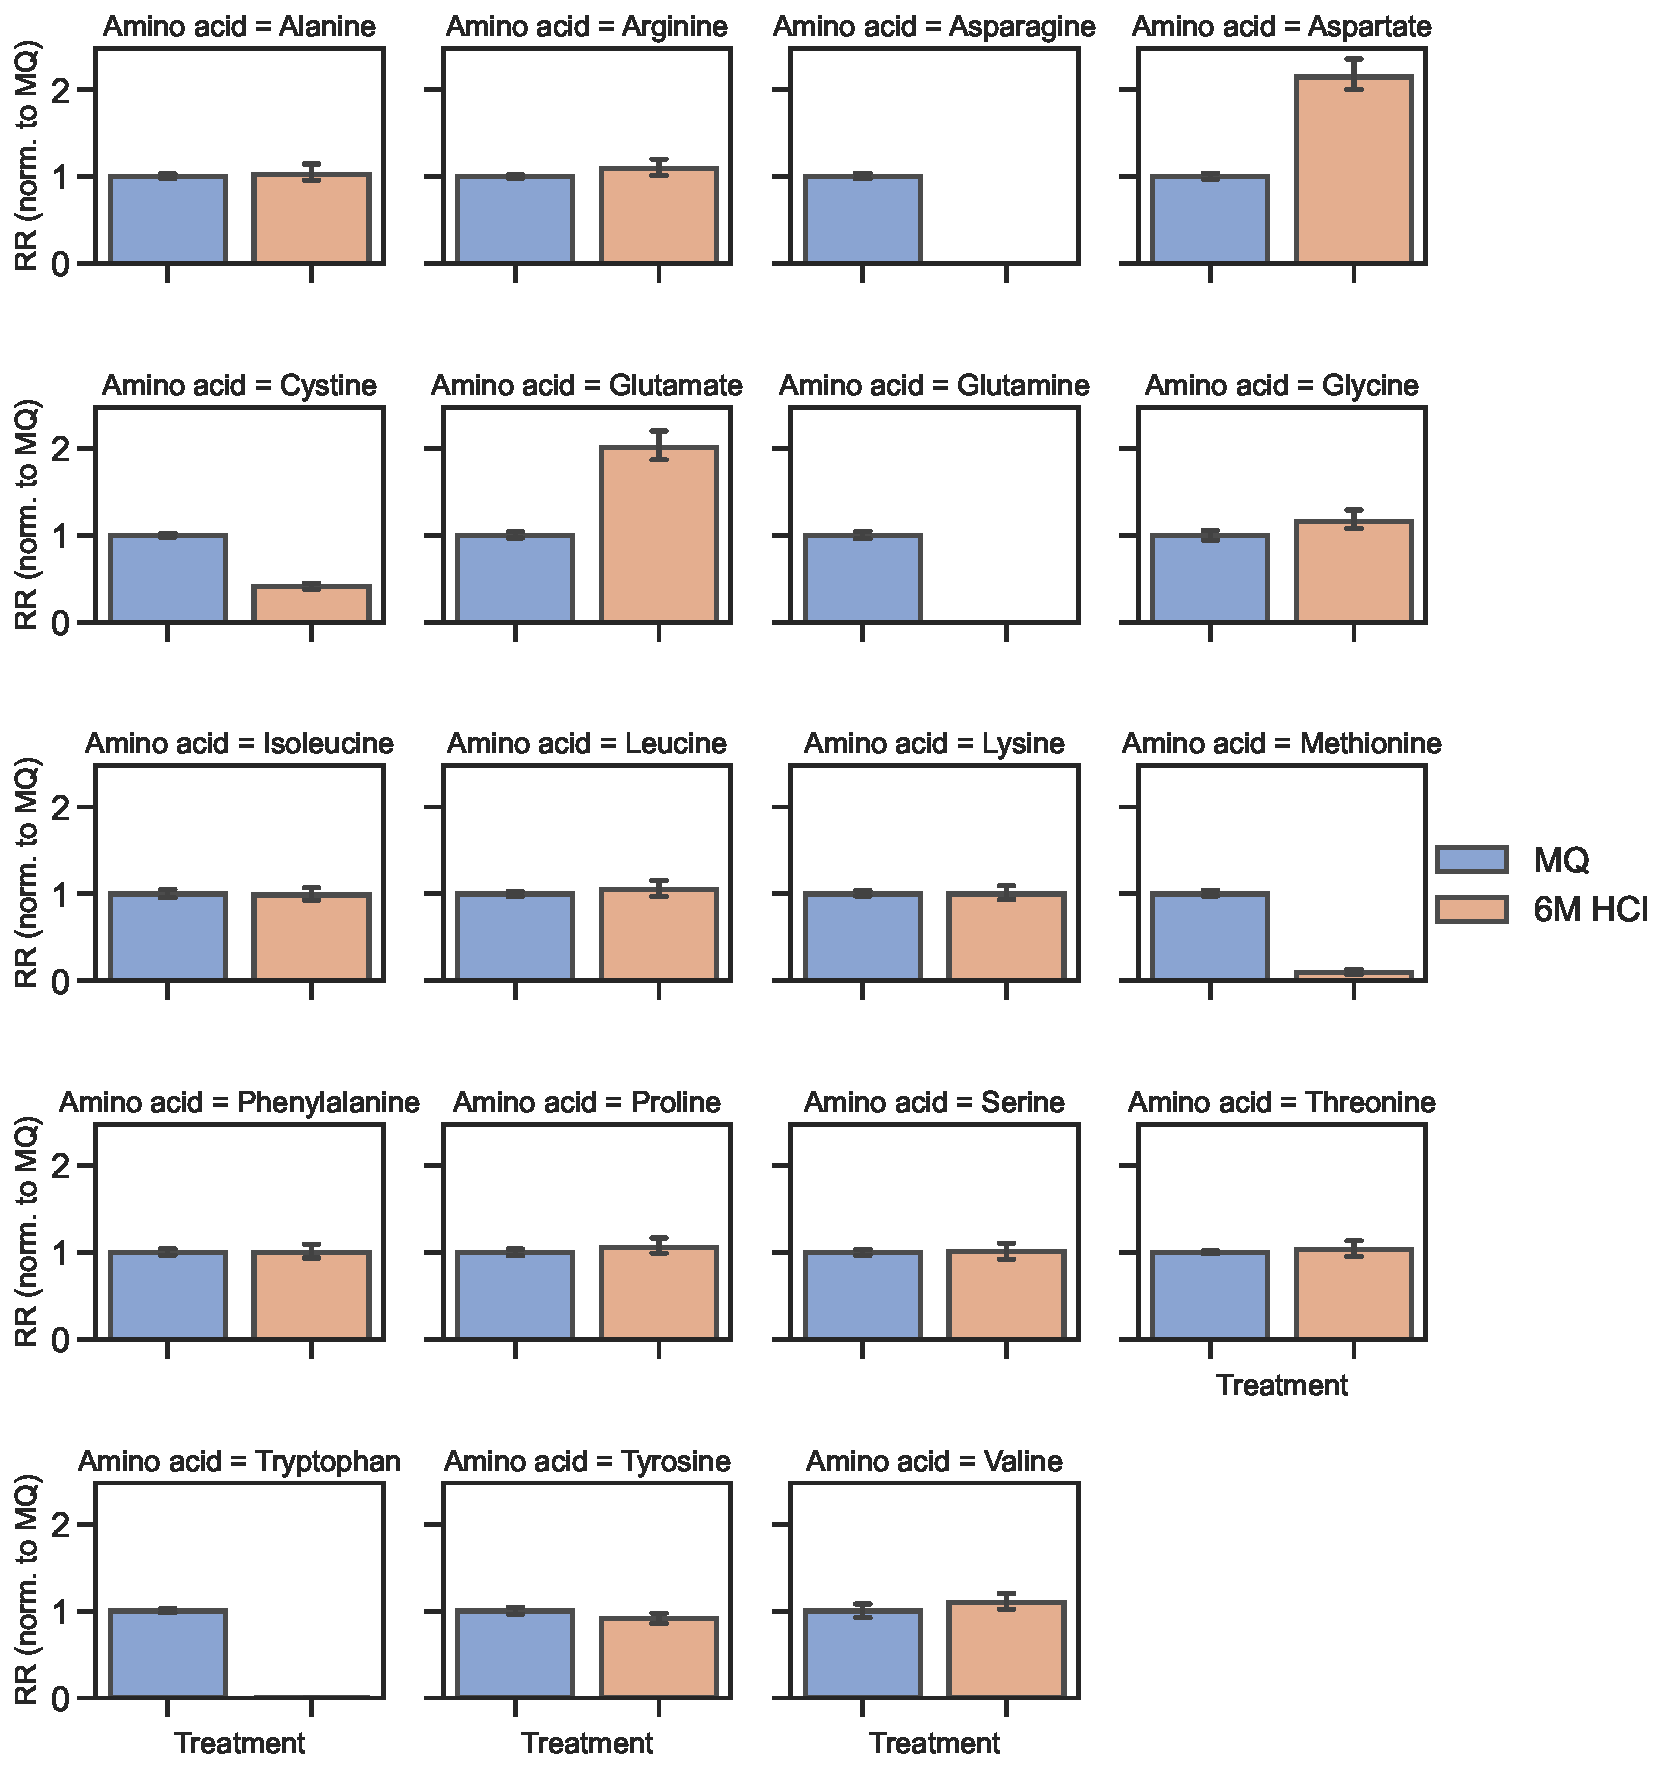
\includegraphics[width=0.95\textwidth]{figures/chap2/app/AA_acid_hydrolysis_stability.pdf}
    \caption[Amino acid stability in HCl.]{
    Amino acid stability in 6 M HCl after 24 hours incubation at 100°C in tubes with ambient air headspace.
    Incubation in HCl was compared with water (MQ).
    Ion counts were normalized to their internal standard (RR, response ratio).
    }
    \label{fig:app_ch2:AA_acid_hydrolysis_stability}
\end{figure}

\begin{figure}[ht]
    \centering
    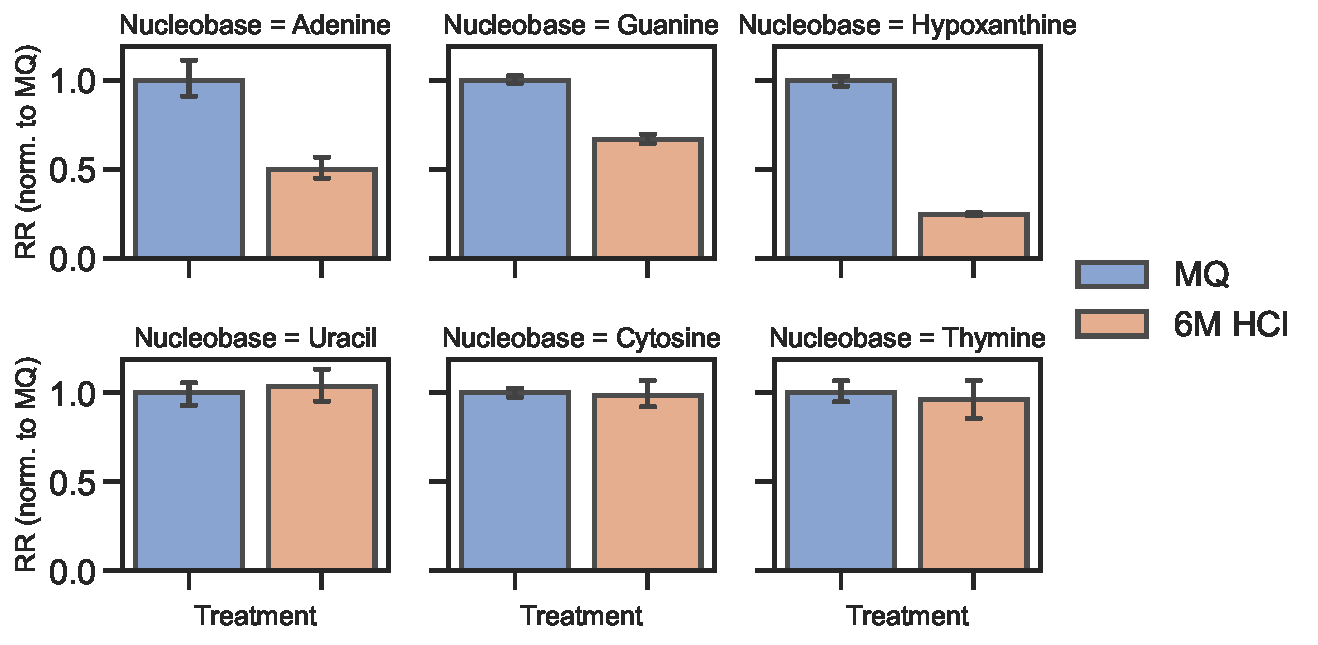
\includegraphics[width=0.8\textwidth]{figures/chap2/app/nucleobase_hydrolysis_stability.pdf}
    \caption[Nucleobase stability in HCl.]{
    Nucleobase stability in 6 M HCl after 24 hours incubation at 100°C in tubes with ambient air headspace.
    Incubation in HCl was compared with water (MQ).
    Ion counts were normalized to their internal standard (RR, response ratio).
    }
    \label{fig:app_ch2:nucleobase_hydrolysis_stability}
\end{figure}

\begin{figure}[ht]
     \centering
     \begin{subfigure}[b]{0.49\textwidth}
         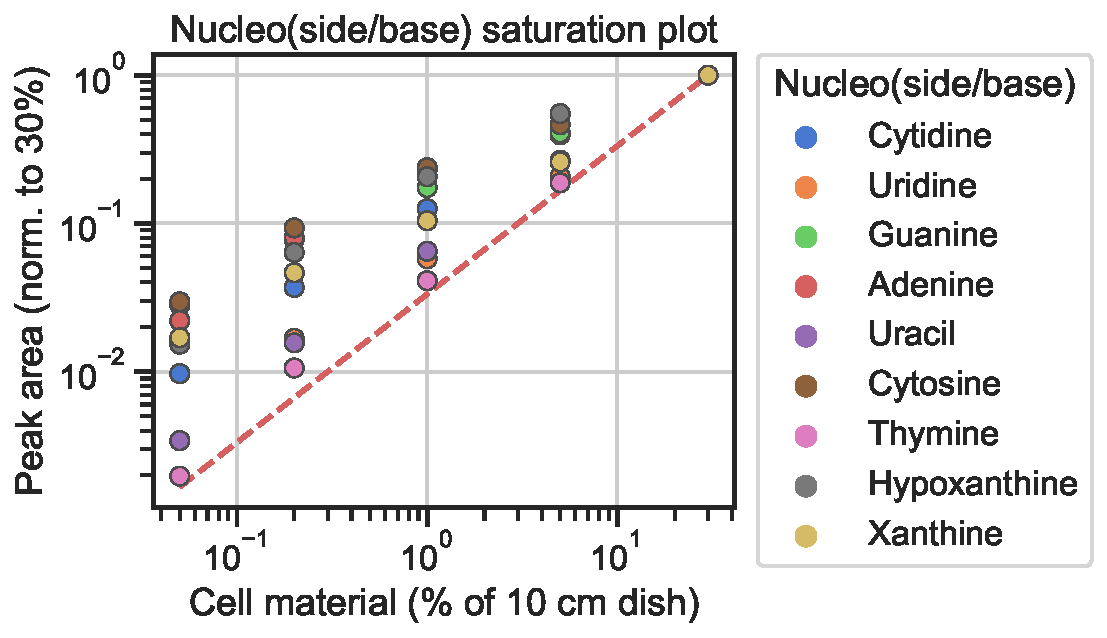
\includegraphics[width=\textwidth]{figures/chap2/app/hydrolysis_nucl_saturation.pdf}
     \end{subfigure}
     \hfill
     \begin{subfigure}[b]{0.49\textwidth}
         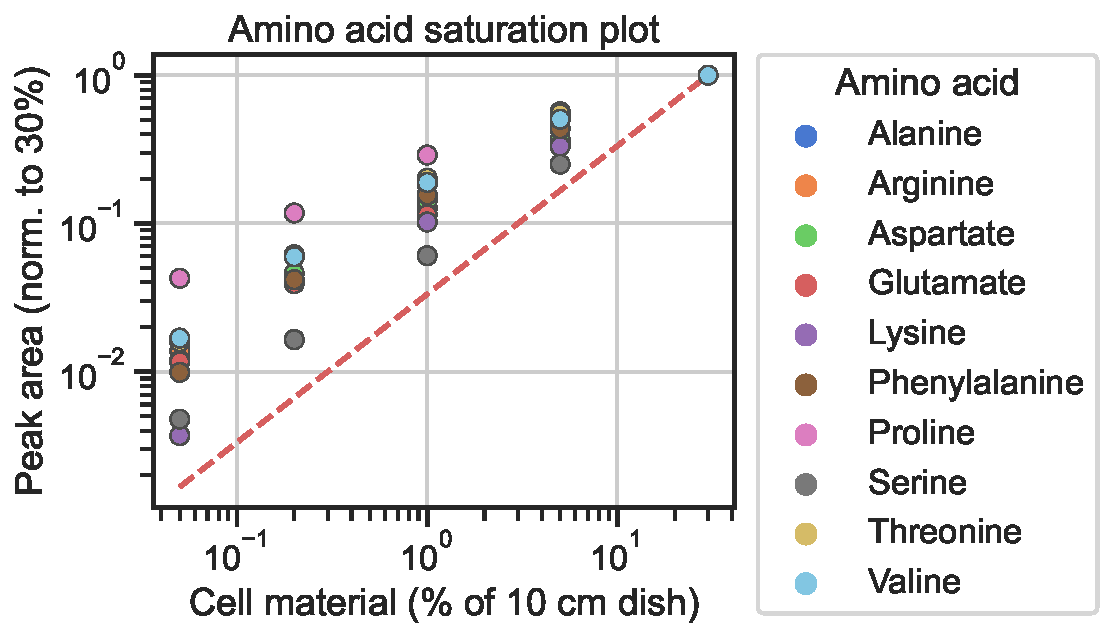
\includegraphics[width=\textwidth]{figures/chap2/app/hydrolysis_AA_saturation.pdf}
     \end{subfigure}
        \caption[Nucleoside, nucleobase and amino acid, hydrolysis saturation.]{
        LCMS measured peak area of nucleosides, nucleobases (left) and amino acids (right) using increasing amounts of cell material as input for acid hydrolysis.
        The increase in cell material results in an increase in peak area for all compounds, indicating that none have reached their solubility limit.
        The red dashed line shows direct proportionality using the 30\% cell material as reference.
        Points above the this line indicate ion suppression.
        }
        \label{fig:app_ch2:hydrolysis_saturation}
\end{figure}

\begin{figure}[ht]
    \centering
    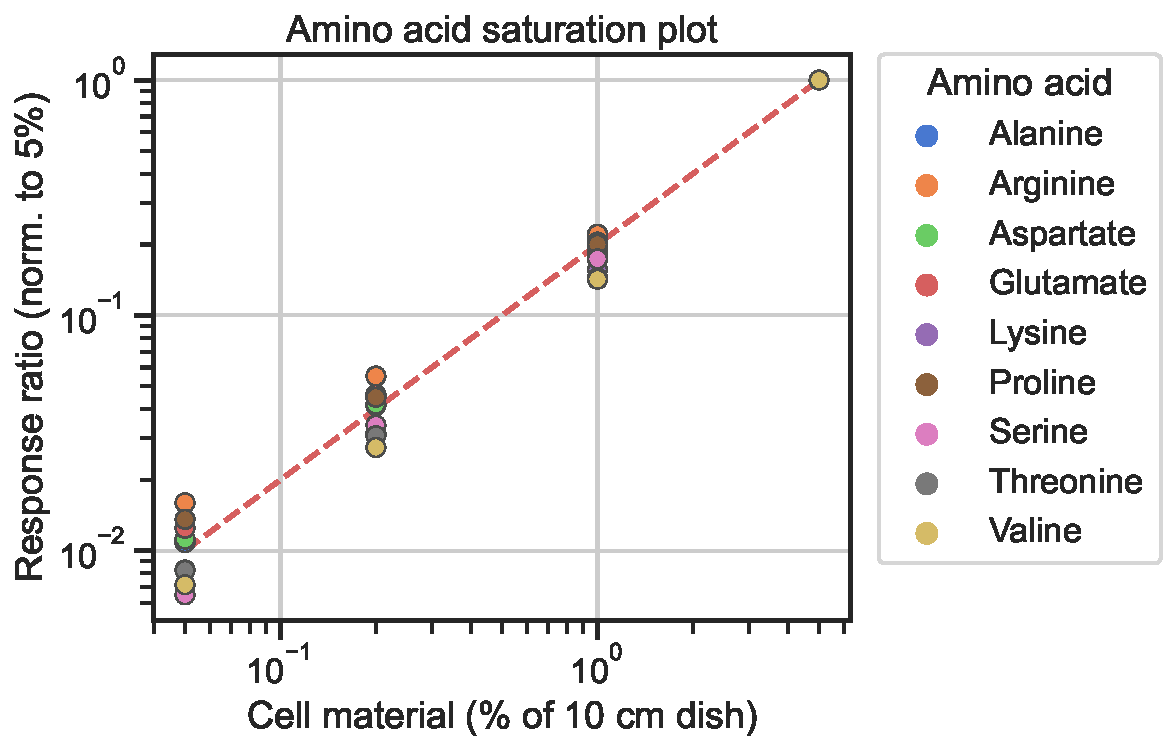
\includegraphics[width=0.49\textwidth]{figures/chap2/app/hydrolysis_AA_saturation_RR.pdf}
    \caption[Hydrolyzed amino acids normalized with internal standards.]{
    Ion suppression observed in the above figure \ref{fig:app_ch2:hydrolysis_saturation} (right panel) can be removed by normalization to the isotopically labelled internal standard for each compound.
    }
    \label{fig:app_ch2:hydrolysis_AA_saturation_RR}
\end{figure}

% KD: No reason to include this as this was mostly testing the reproducibility of transfering cell material equally to each replicate sample. Later on-plate hydrolysis was used and the transfer of cell material is not an issue.
%The reproducibility of the whole quantification process was tested by preparing four samples run in parallel 
%\begin{figure}[ht]
%    \centering
%    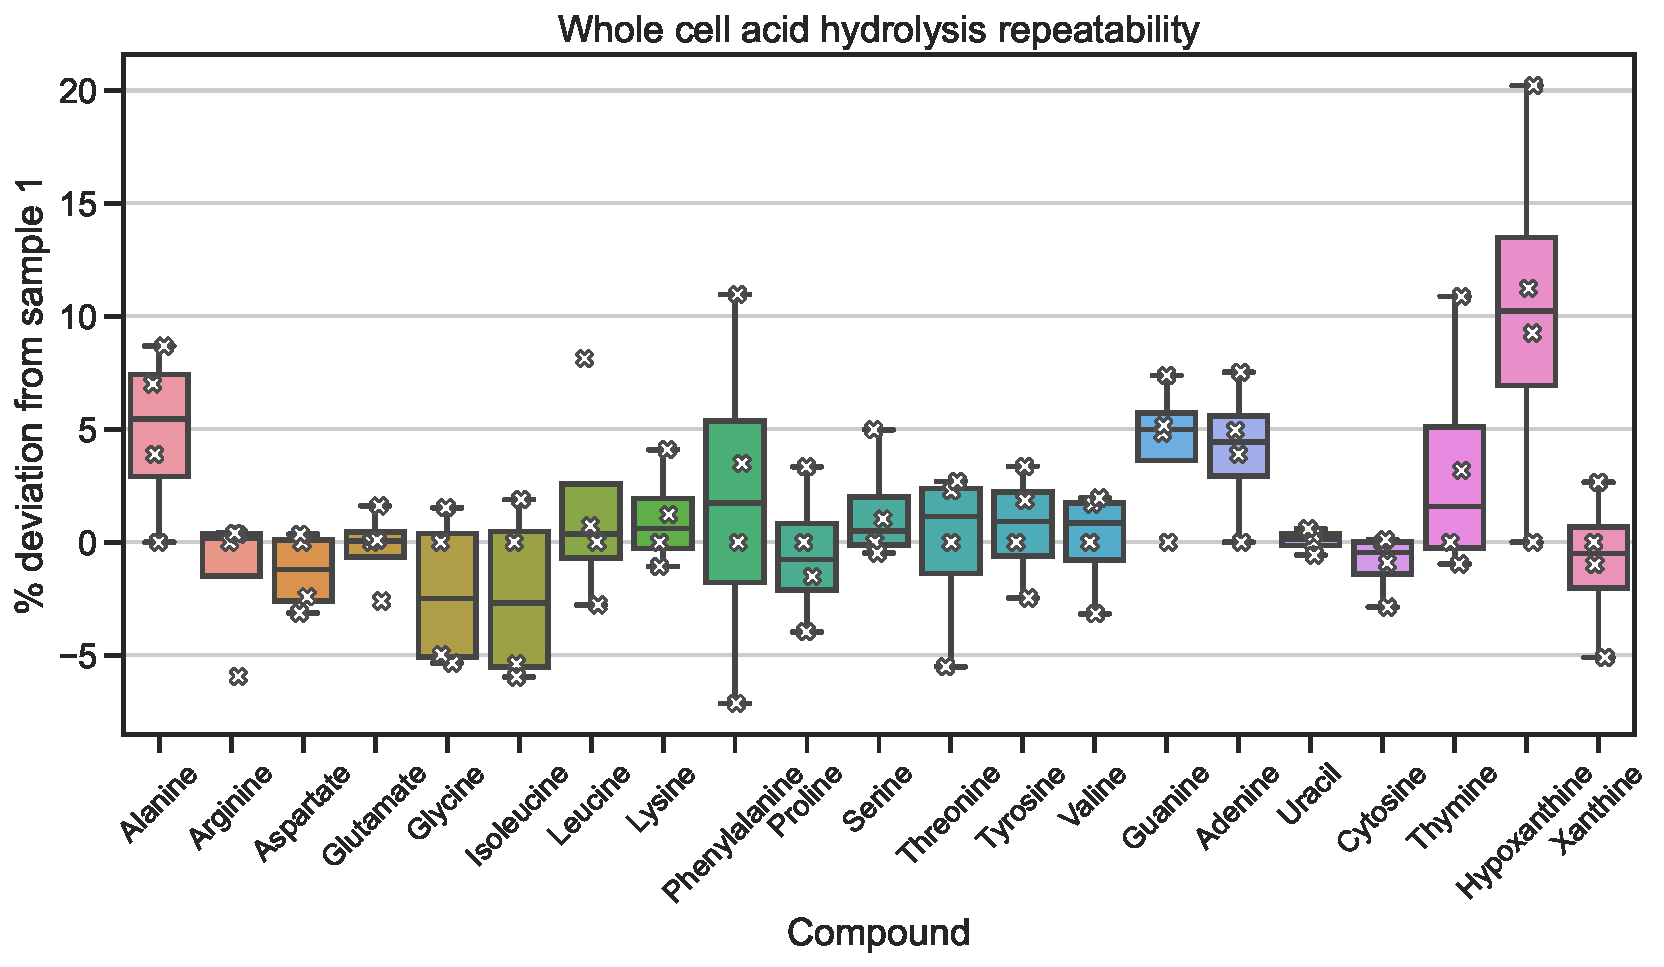
\includegraphics[width=0.7\textwidth]{figures/chap2/app/hydrolysis_repeatability.pdf}
%    \caption[Cell hydrolysis repeatability.]{
%    qwertyu
%    }
%    \label{fig:app_ch2:hydrolysis_repeatability}
%\end{figure}

\begin{figure}[ht]
     \centering
     \begin{subfigure}[b]{0.4\textwidth}
         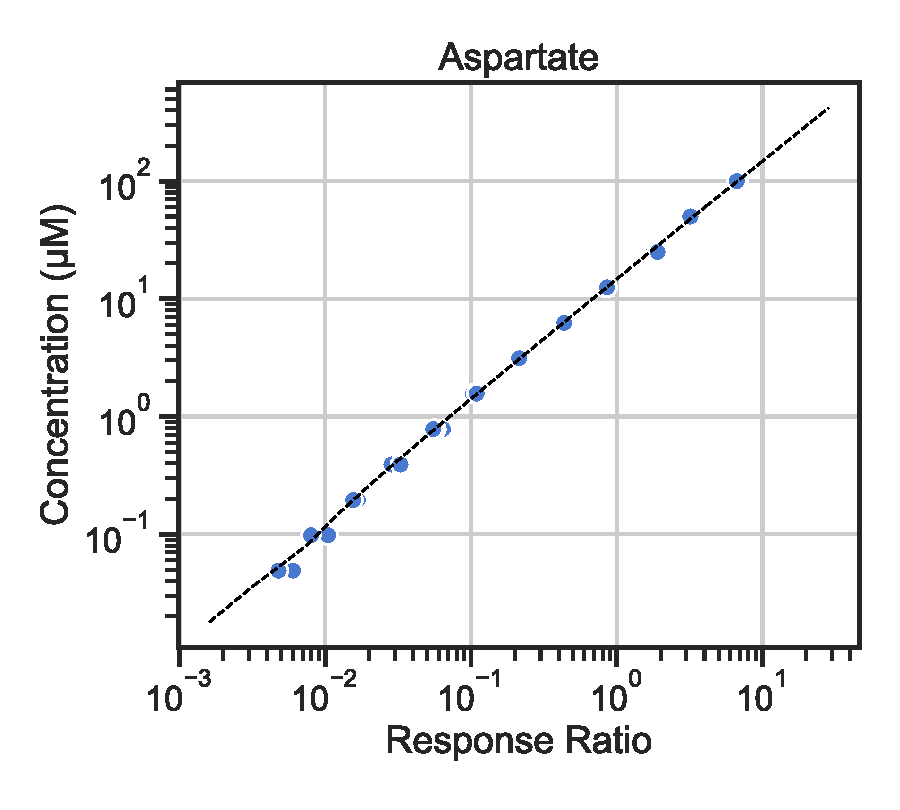
\includegraphics[width=\textwidth]{figures/chap2/app/calibration_curve_asp.pdf}
     \end{subfigure}
     %\hfill
     \hspace{0.035\textwidth}
     \begin{subfigure}[b]{0.4\textwidth}
         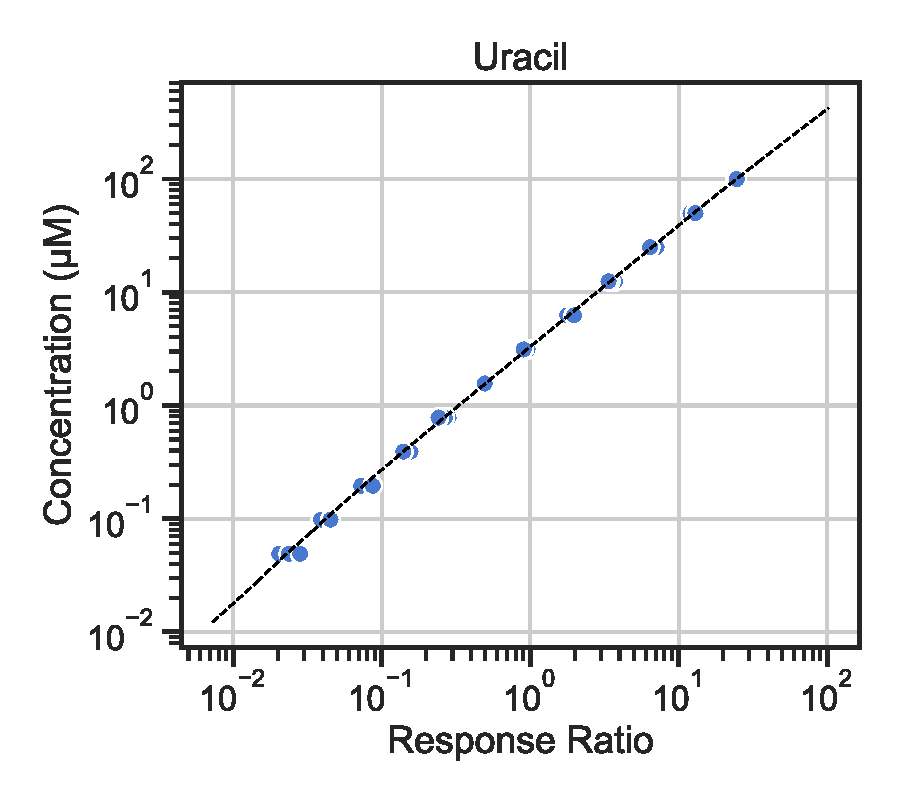
\includegraphics[width=\textwidth]{figures/chap2/app/calibration_curve_uracil.pdf}
     \end{subfigure}
        \caption[Isotope dilution calibration curves.]{
        Examples of calibration curves fitted to three replicates of a compound titration spanning three orders of magnitude.
        }
        \label{fig:app_ch2:calibration_curve}
\end{figure}




\section{15N Gln tracing in 143B and H1299}
\begin{figure}[ht]
    \centering
    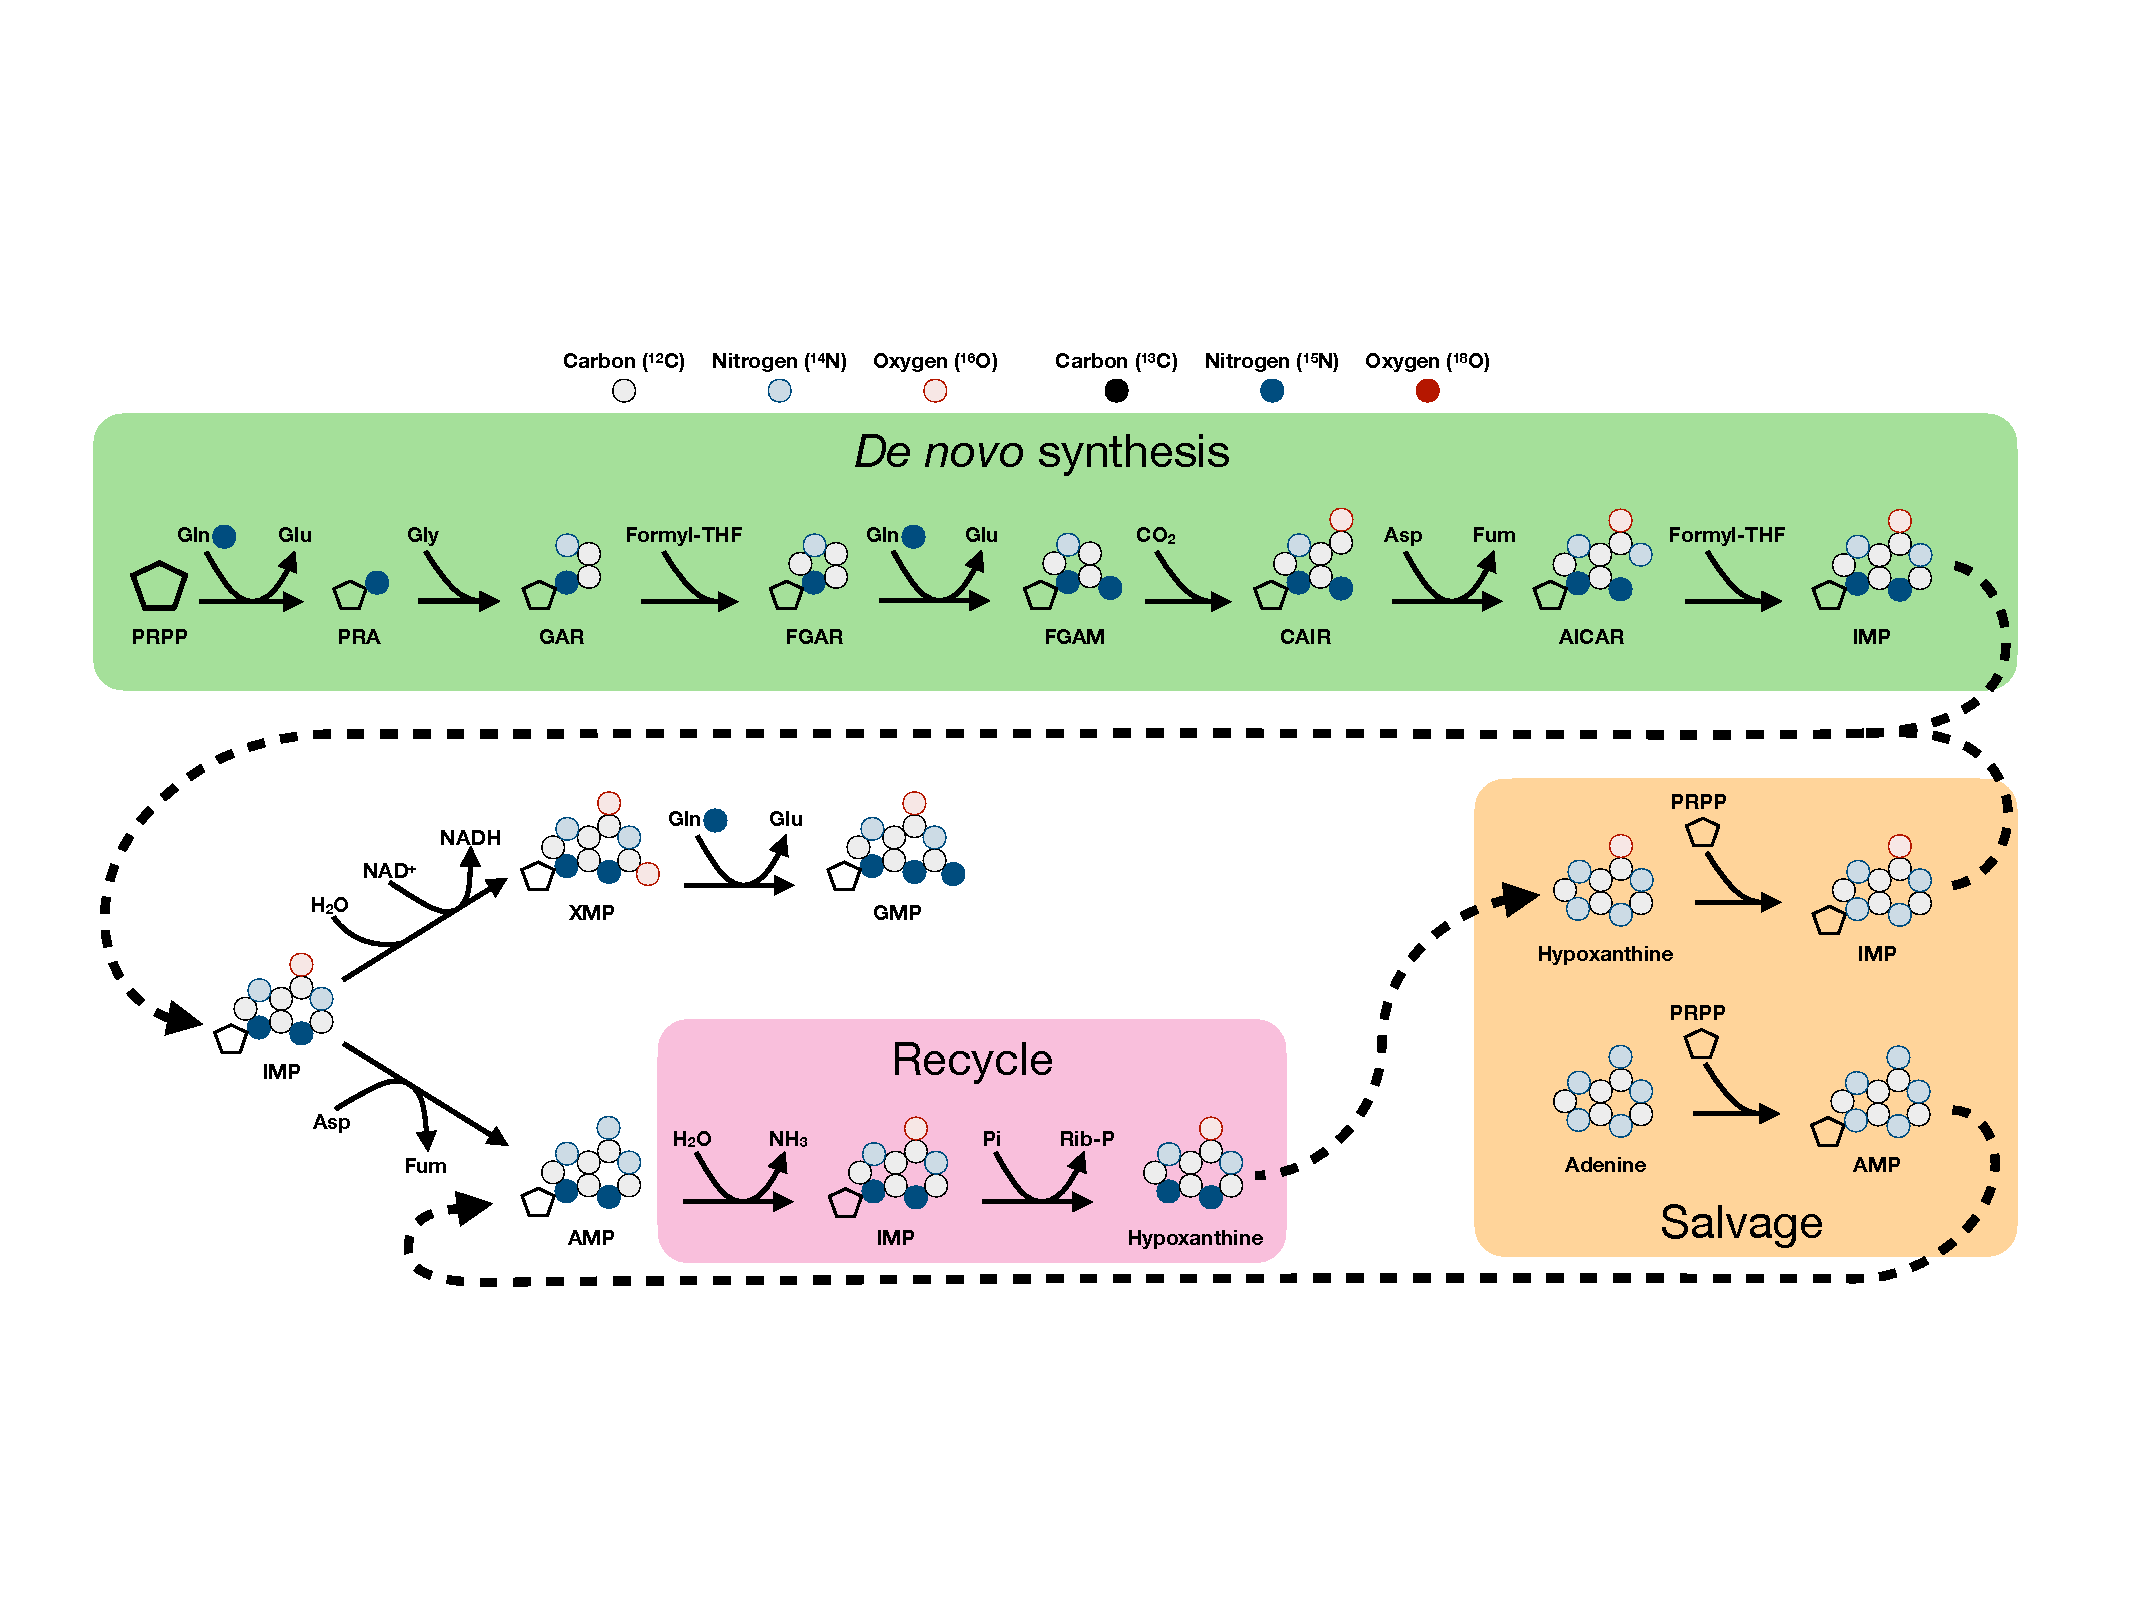
\includegraphics[width=0.95\textwidth]{figures/chap2/app/purine_tracing_overvew.pdf}
    \caption[Purine metabolism \hNi-amide Gln tracing overview.]{
    Overview of Gln \hNi-amide label incorporation in \textit{de novo} purine synthesis.
    Label incorporation can be effected by salvage of unlabelled hypoxanthine or adenine and recycling.
    }
    \label{fig:app_ch2:pur_tr_ov}
\end{figure}

\begin{figure}
    \centering
    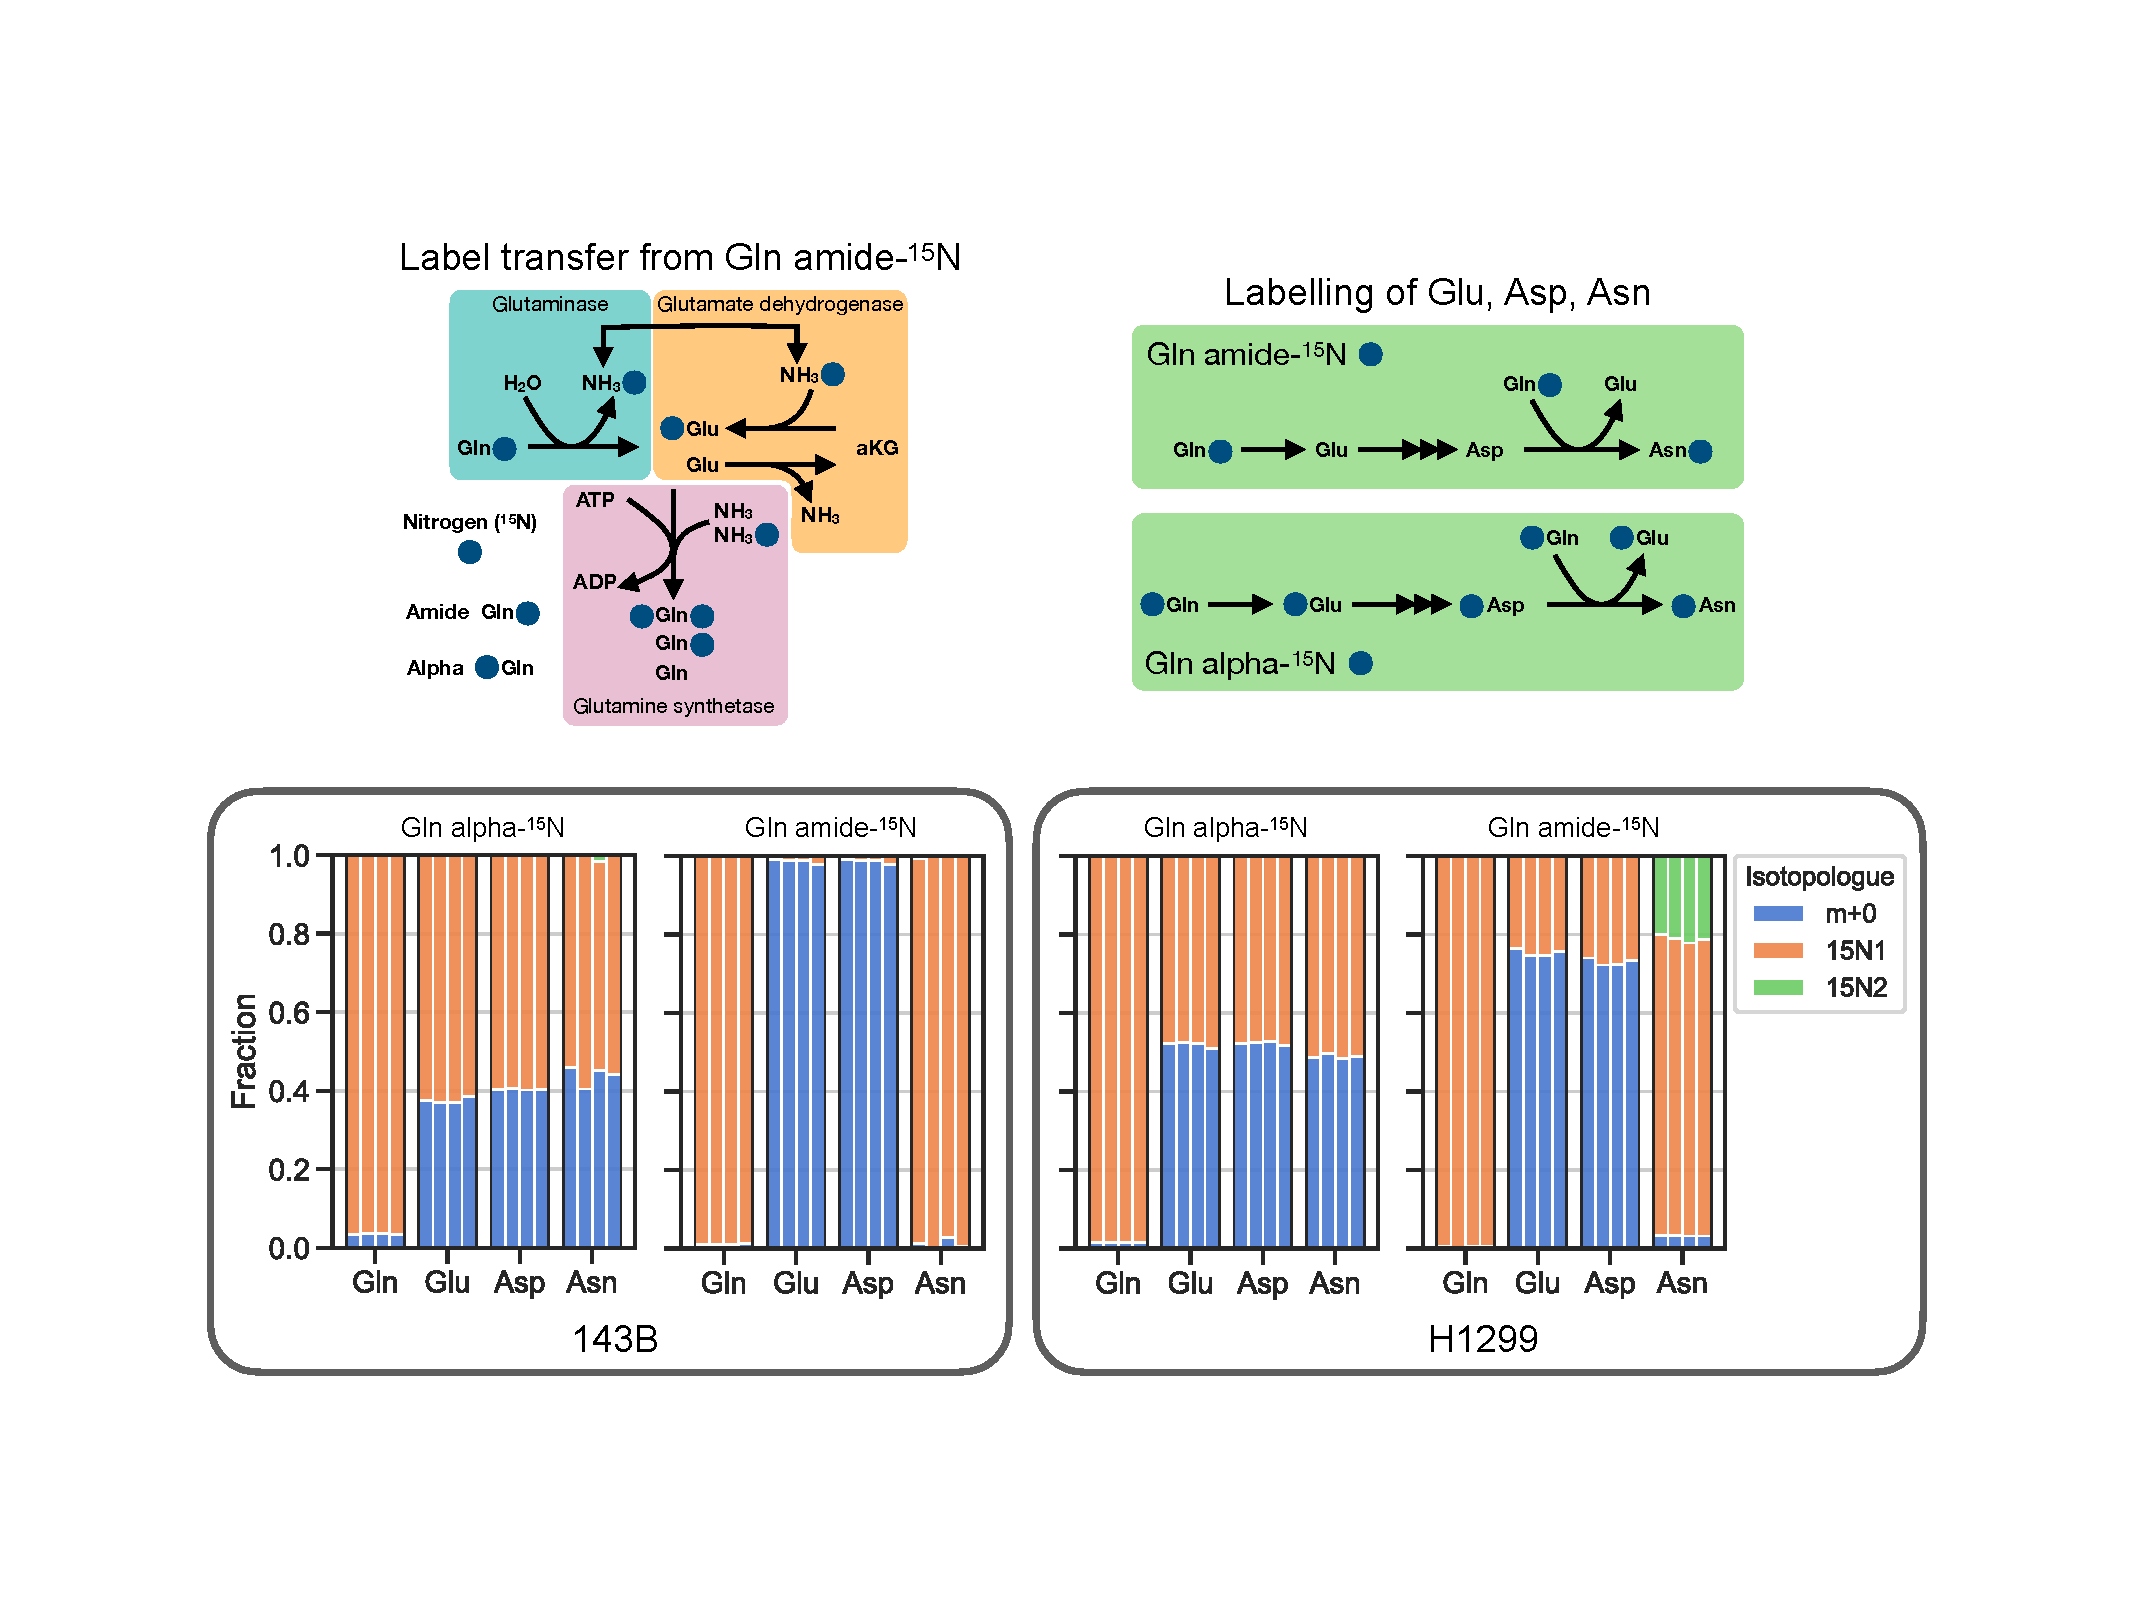
\includegraphics[width=0.95\textwidth]{figures/chap2/app/gln_lab_tranfr.pdf}
    \caption[Gln amide to alpha \hNi{} transfer.]{
    Gln \hNi{} on the amide nitrogen can transfer to the alpha nitrogen in H1299 cells but not in 143B cells.
    Upper left diagram shows how Gln amide and alpha nitrogen labels can transfer.
    Transfer of amide labelled nitrogen can be achieved by glutaminase catalyzed release of labelled ammonia and its subsequent use as a substrate in the conversion of alpha-ketoglutarate (aKG) to Glu alpha-\hNi{} by glutamate dehydrogenase.
    The signature of glutamine synthetase activity is the appearance of doubly labelled Gln.
    Upper right diagram shows how Gln amide and alpha nitrogen labels are transferred to downstream metabolites Glu, Asp and Asn.
    Lower panel shows the nitrogen isotopologue distribution of Gln, Glu, Asp and Asn in 143B and H1299 at steady-state.
    The alpha nitrogen label is frequently lost in Glu and downstream, presumably due to transaminase catalyzed exchange with unlabelled amino groups on amino acids such as leucine, isoleucine, valine etc.
    The amide nitrogen label is partially transferred to the alpha position in H1299, but not in 143B, also indicated by the doubly labelled Asn.
    }
    \label{fig:app_ch2:gln_lab_tranfr}
\end{figure}

\begin{figure}[ht]
     \centering
     \begin{subfigure}[b]{0.4\textwidth}
         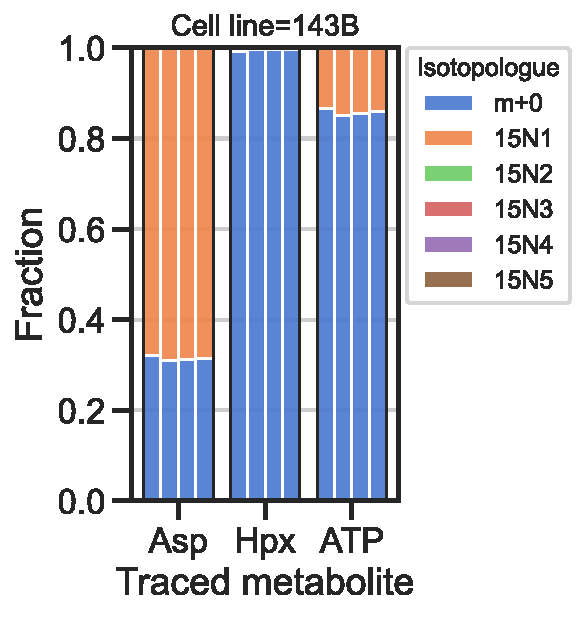
\includegraphics[width=\textwidth]{figures/chap2/app/Ade-sal_143B.pdf}
         \caption{}
         \label{fig:app_ch2:ade_sal_143B}
     \end{subfigure}
     %\hfill
     \hspace{0.015\textwidth}
     \begin{subfigure}[b]{0.4\textwidth}
         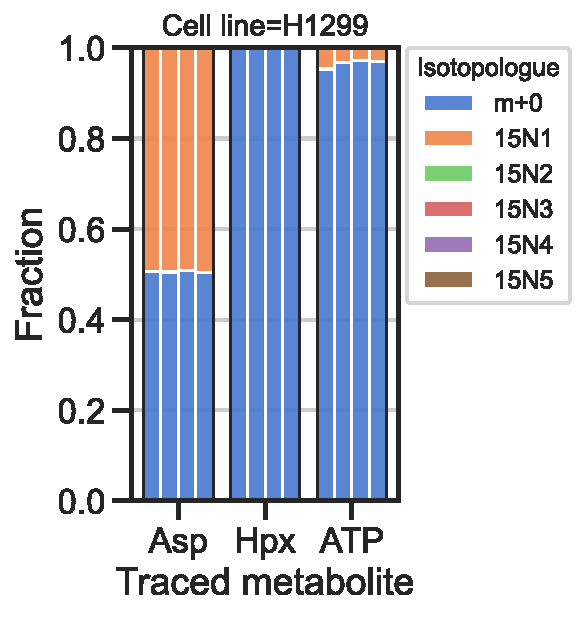
\includegraphics[width=\textwidth]{figures/chap2/app/Ade-sal_H1299.pdf}
         \caption{}
         \label{fig:app_ch2:ade_sal_H1299}
     \end{subfigure}
        \caption[Glu alpha-\hNi{} tracing into Asp, Hpx and ATP.]{
        Glu alpha-\hNi{} tracing into Asp, Hpx and ATP at steady-state for cell lines 143B and H1299 grown in DMEM with 100 µM adenine.
        \textit{De novo} ATP synthesis and salvage from Hpx results in label incorporation from Asp, while salvage from adenine does not (figure \ref{fig:app_ch2:pur_tr_ov}).
        Therefore, the salvage fraction directly from adenine can be inferred from the fold difference of Asp vs. ATP labelling.
        }
        \label{fig:app_ch2:ade_sal}
\end{figure}

\begin{figure}[ht]
    \centering
    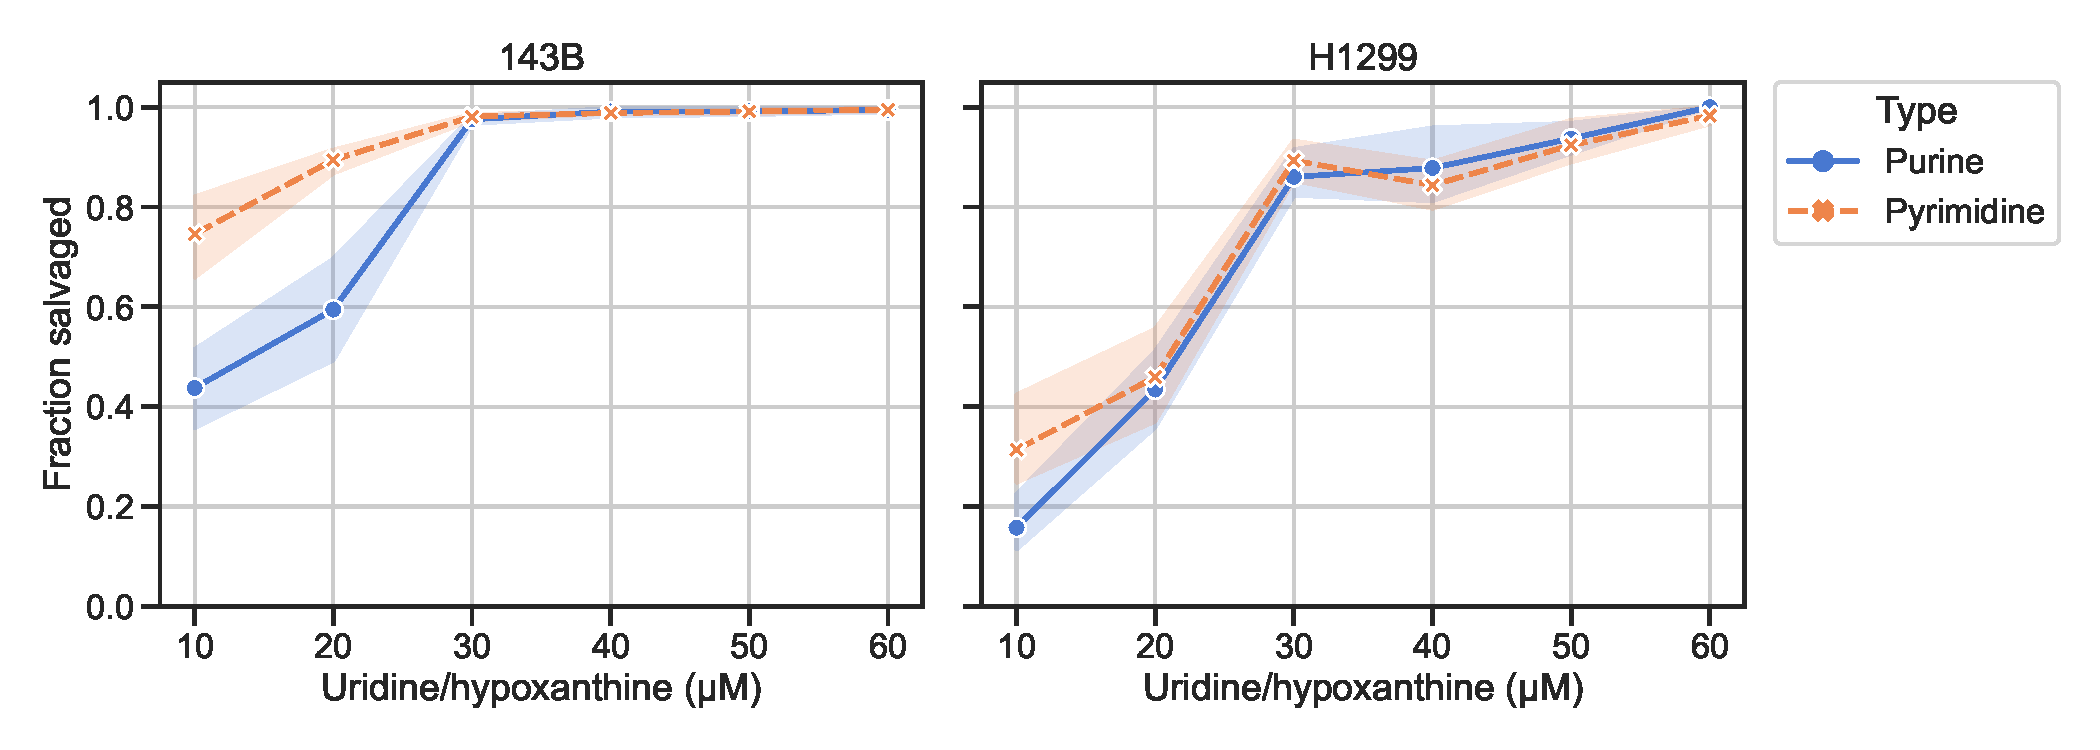
\includegraphics[width=0.95\textwidth]{figures/chap2/app/sal_frac_conc.pdf}
    \caption[Salvage as a function of Urd/Hpx concentration.]{
    Fraction of purines (average across GDP, GMP, ADP and AMP) and pyrimidines (average across UDP, UMP, CDP and CMP) derived from salvage when 143B or H1299 cells are cultured in increasing concentrations of uridine/hypoxanthine.
    }
    \label{fig:app_ch2:sal_frac_conc}
\end{figure}

\begin{figure}[ht]
    \centering
    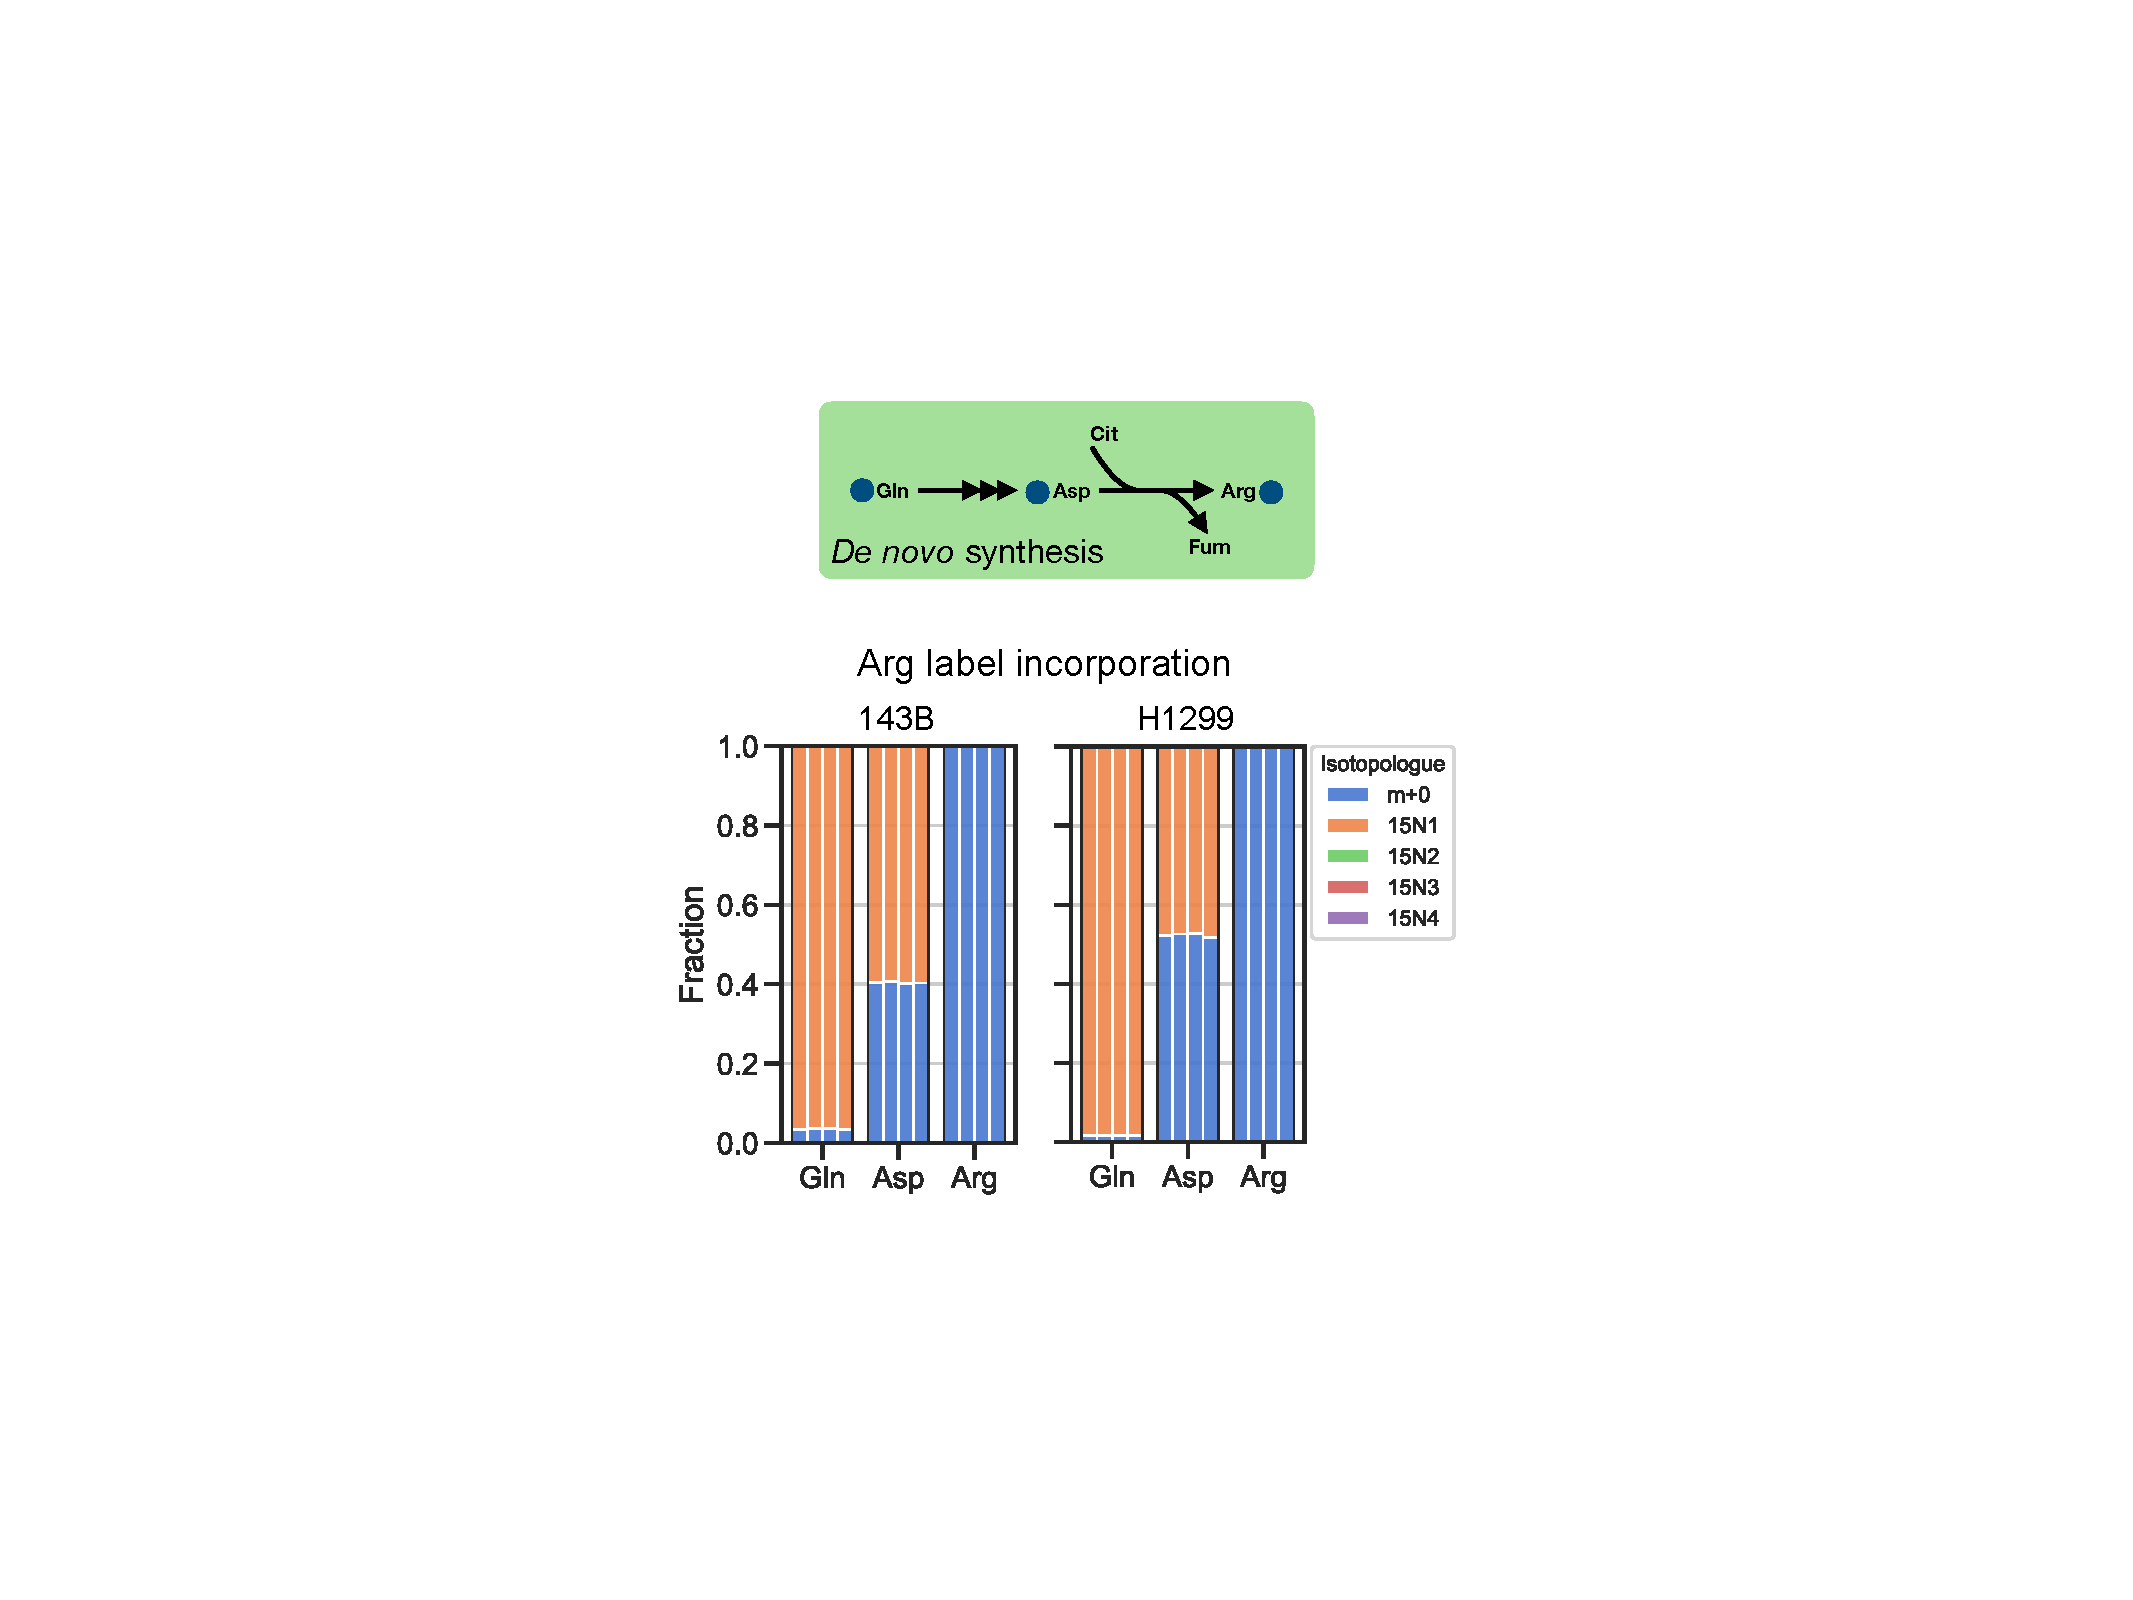
\includegraphics[width=0.45\textwidth]{figures/chap2/app/arg_syn.pdf}
    \caption[No evidence of arginine synthesis in DMEM.]{
    No evidence of arginine synthesis in DMEM.
    Top diagram shows Gln alpha\=/\hNi{} label incorporation into Asp and subsequently Arg.
    Bottom isotopologue distributions show Gln alpha\=/\hNi{} label incorporation into Gln, Asp and Arg at steady-state for cell lines 143B and H1299 grown in DMEM with no salvageable metabolites added (Vec).
    }
    \label{fig:app_ch2:arg_syn}
\end{figure}




\section{ETC inhibitor rescue with purines is blunted in serine free media}
\begin{figure}[ht]
    \centering
    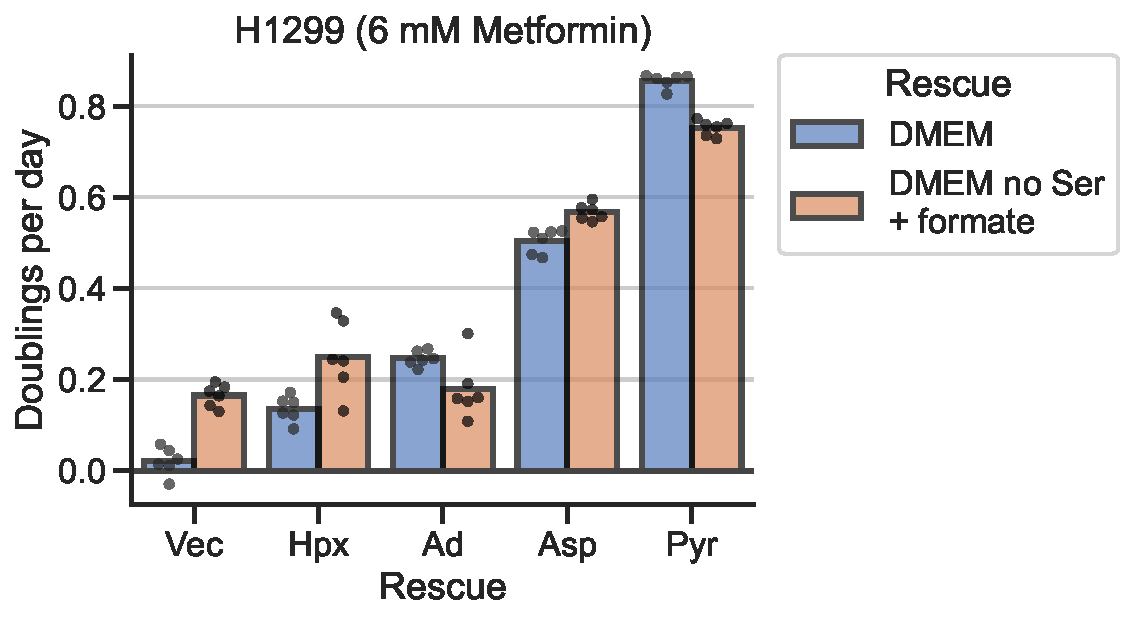
\includegraphics[width=0.6\textwidth]{figures/chap2/app/H1299_Met_rescue_noSer.pdf}
    \caption[ETC inhibitor purine rescue in serine free media.]{
    The small proliferation rescue of hypoxanthine and adenine during 6 mM metformin treatment, is blunted by when repeated in serine free media with 1 mM sodium formate.
    Serine free media will decrease the mitochondria NADH production by the folate cycle; instead, formate becomes necessary to generate folate species e.g. 10-formyl–THF for purine synthesis \cite{Ducker2016-mz, Ducker2017-mb, Yang2020-fs}.
    Related to figure \ref{fig:ch2:H1299_Met_rescue}.
    }
    \label{fig:app_ch2:H1299_Met_rescue_noSer}
\end{figure}




\section{Aspartate to proliferation curves}
\label{sec:ch2:app:asp_prlfr}
\begin{figure}[ht]
     \centering
     \begin{subfigure}[b]{0.49\textwidth}
         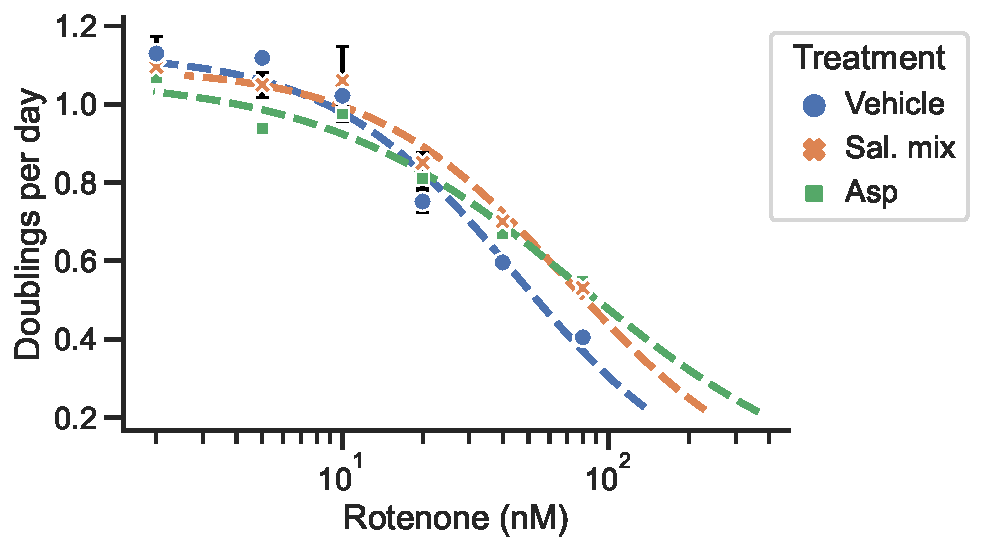
\includegraphics[width=\textwidth]{figures/chap2/app/H1299_Rot_Rot_vs_prlfr_noPyr.pdf}
         \caption{}
         \label{fig:app_ch2:H1299_Rot_Rot_vs_prlfr}
     \end{subfigure}
     \hfill
     \begin{subfigure}[b]{0.49\textwidth}
         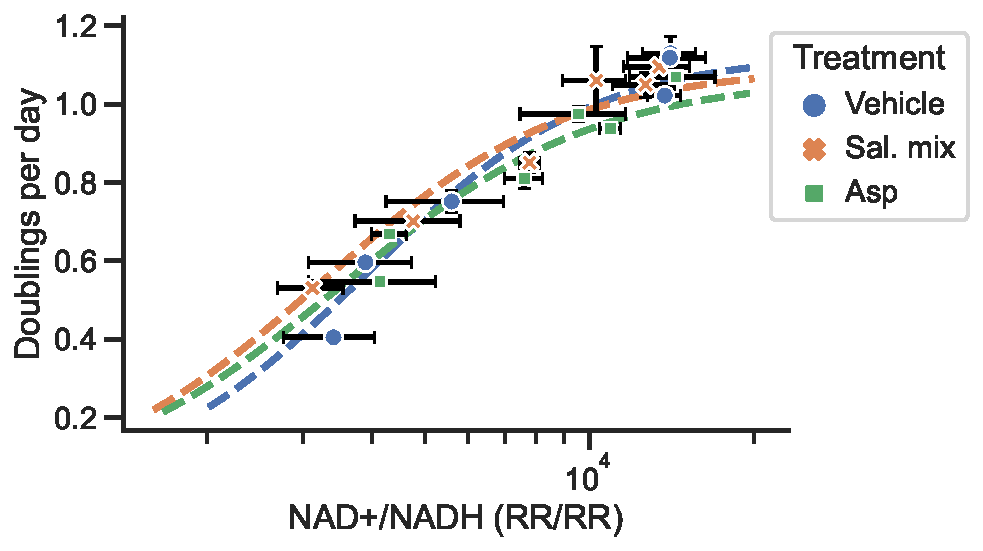
\includegraphics[width=\textwidth]{figures/chap2/app/H1299_Rot_NAD_vs_prlfr_noPyr.pdf}
         \caption{}
         \label{fig:app_ch2:H1299_Rot_NAD_vs_prlfr}
     \end{subfigure}
        \caption[H1299 rotenone titration aspartate to proliferation.]{
        Supplementary data for figure \ref{fig:ch2:H1299_Rot_Asp_vs_prlfr}.
        (a) Proliferation as a function of rotenone concentration.
        Rotenone concentration at 50\% proliferation is 40, 70 and 80 nM for Vehicle, Sal. mix and Asp treatments, respectively.
        (b) Proliferation as a function of the \NAD{}/NADH ratio.
        The \NAD{}/NADH ratio was made using internal standard normalized LCMS measurements (response ratio/response ratio).
        Condition with salvage mix (Sal. mix) contains: 1 mM asparagine/uridine, 0.5 mM hypoxanthine, 20 µM adenine and 10 µM adenosine.
        }
        \label{fig:app_ch2:H1299_Rot_RotNAD_vs_prlfr}
\end{figure}

\begin{figure}[ht]
     \centering
     \begin{subfigure}[b]{0.49\textwidth}
         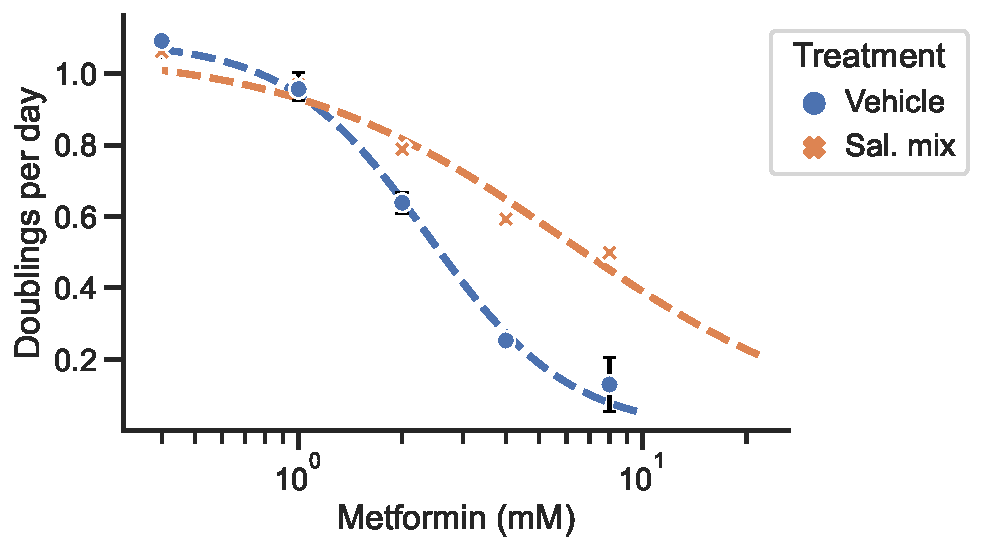
\includegraphics[width=\textwidth]{figures/chap2/app/H1299_Met_Met_vs_prlfr.pdf}
         \caption{}
         \label{fig:app_ch2:H1299_Met_Met_vs_prlfr}
     \end{subfigure}
     \hspace{0.255\textwidth}
     \begin{subfigure}[b]{0.49\textwidth}
         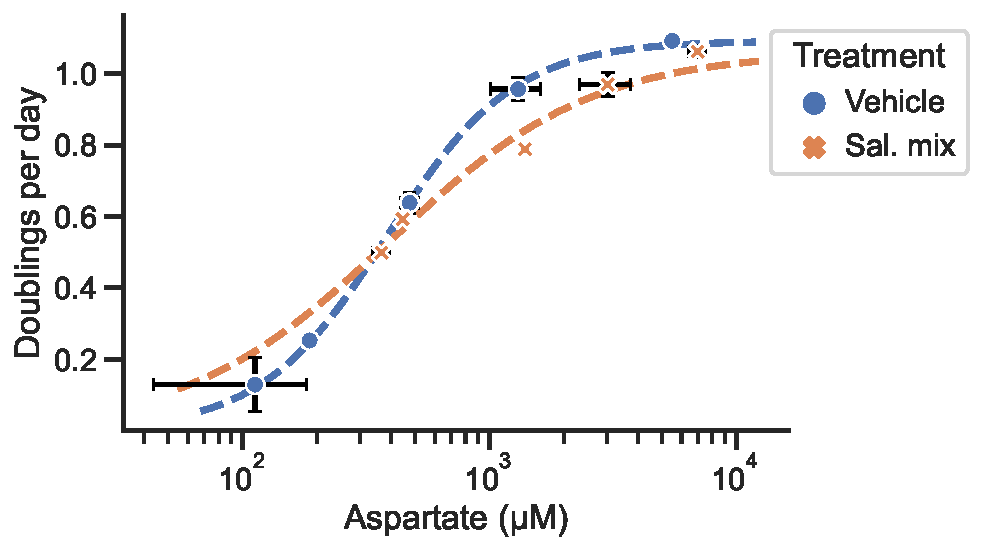
\includegraphics[width=\textwidth]{figures/chap2/app/H1299_Met_Asp_vs_prlfr.pdf}
         \caption{}
         \label{fig:app_ch2:H1299_Met_Asp_vs_prlfr}
     \end{subfigure}
     \hfill
     \begin{subfigure}[b]{0.49\textwidth}
         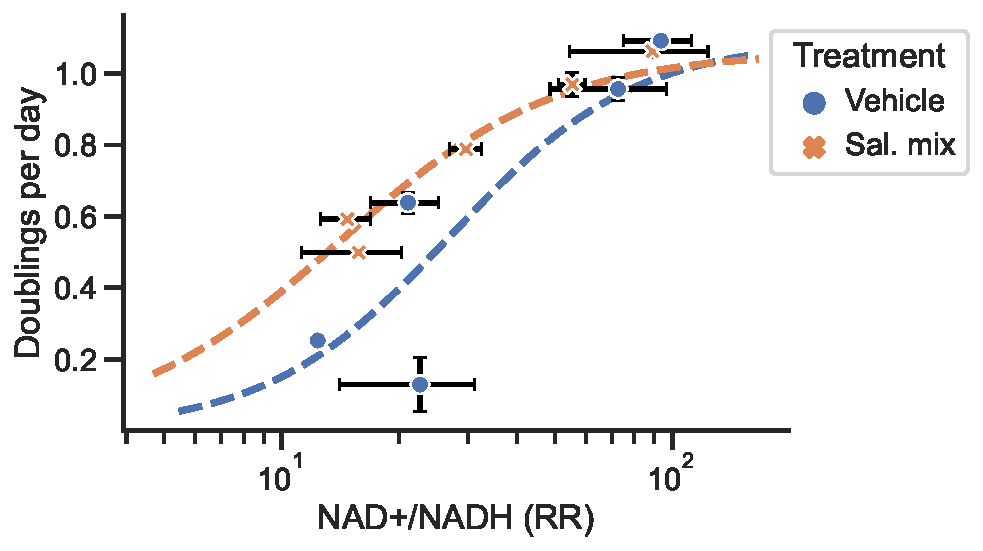
\includegraphics[width=\textwidth]{figures/chap2/app/H1299_Met_NAD_vs_prlfr.pdf}
         \caption{}
         \label{fig:app_ch2:H1299_Met_NAD_vs_prlfr}
     \end{subfigure}
        \caption[H1299 metformin titration aspartate to proliferation.]{
        Aspartate to proliferation relationship for H1299 using metformin to induce aspartate limitation.
        (a) Proliferation as a function of metformin concentration.
        Metformin concentration at 50\% proliferation is 2.4 and 6.1 mM for Vehicle and Sal. mix treatments, respectively.
        (b) Proliferation as a function of aspartate concentration.
        Aspartate concentration at 50\% proliferation is 390 µM for both Vehicle and Sal. mix treatments.
        (c) Proliferation as a function of the \NAD{}/NADH ratio.
        The \NAD{}/NADH ratio was made using internal standard normalized LCMS measurements (response ratio/response ratio).
        Condition with salvage mix (Sal. mix) contains: 1 mM asparagine/uridine, 0.5 mM hypoxanthine, 20 µM adenine and 10 µM adenosine.
        }
        \label{fig:app_ch2:H1299_asp_prlfr_met}
\end{figure}

\begin{figure}[ht]
     \centering
     \begin{subfigure}[b]{0.49\textwidth}
         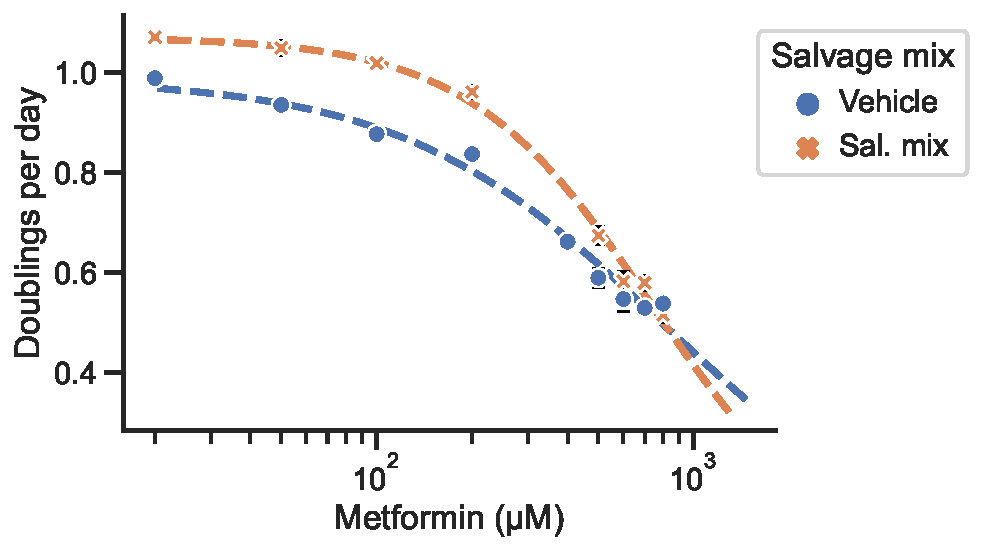
\includegraphics[width=\textwidth]{figures/chap2/app/HCT116_Met_Met_vs_prlfr.pdf}
         \caption{}
         \label{fig:app_ch2:HCT116_Met_Met_vs_prlfr}
     \end{subfigure}
     \hspace{0.255\textwidth}
     \begin{subfigure}[b]{0.49\textwidth}
         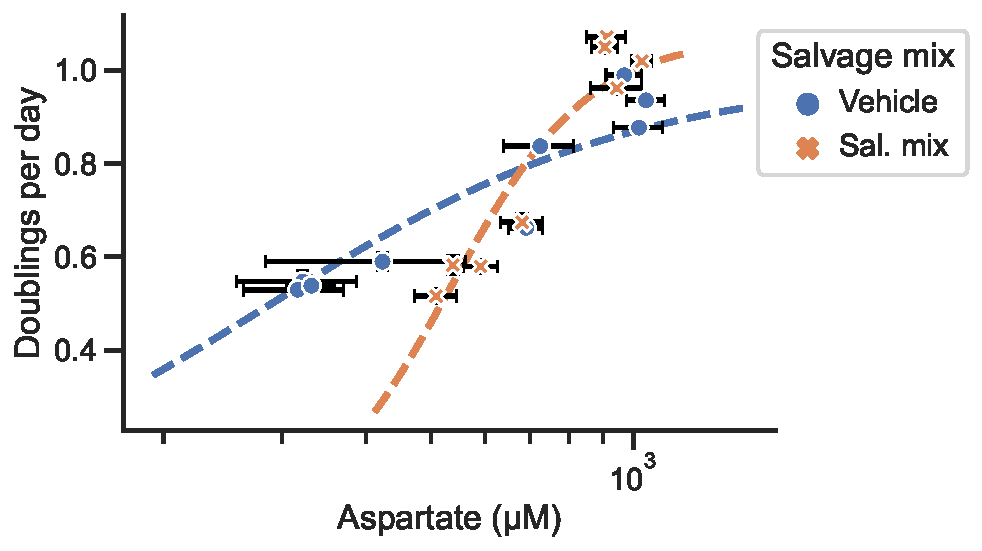
\includegraphics[width=\textwidth]{figures/chap2/app/HCT116_Met_Asp_vs_prlfr.pdf}
         \caption{}
         \label{fig:app_ch2:HCT116_Met_Asp_vs_prlfr}
     \end{subfigure}
     \hfill
     \begin{subfigure}[b]{0.49\textwidth}
         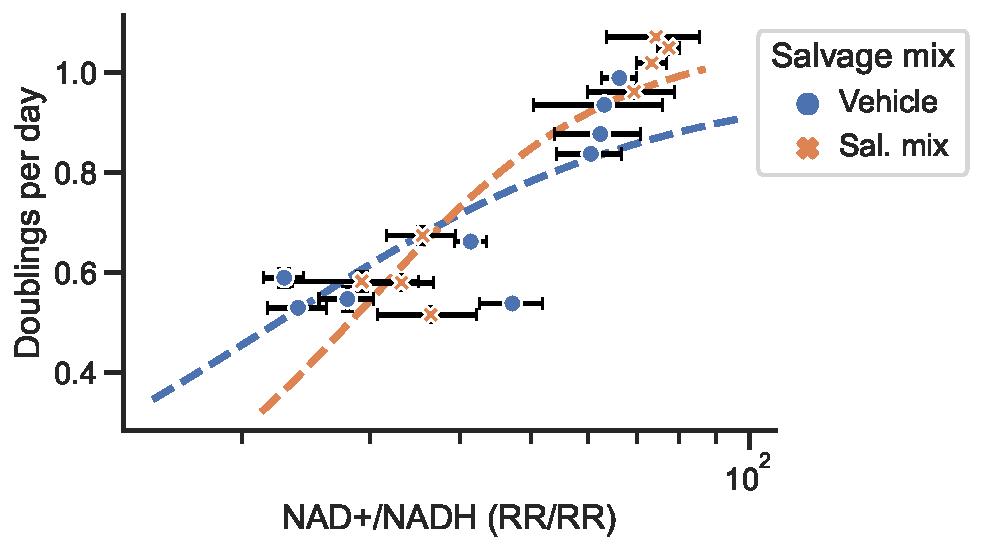
\includegraphics[width=\textwidth]{figures/chap2/app/HCT116_Met_NAD_vs_prlfr.pdf}
         \caption{}
         \label{fig:app_ch2:HCT116_Met_NAD_vs_prlfr}
     \end{subfigure}
        \caption[HCT116 metformin titration aspartate to proliferation.]{
        Aspartate to proliferation relationship for HCT116 using metformin to induce aspartate limitation.
        (a) Proliferation as a function of metformin concentration.
        Metformin concentration at 50\% proliferation is 810 and 740 µM for Vehicle and Sal. mix treatments, respectively.
        (b) Proliferation as a function of aspartate concentration.
        Aspartate concentration at 50\% proliferation is 290 and 530 µM for Vehicle and Sal. mix treatments, respectively.
        (c) Proliferation as a function of the \NAD{}/NADH ratio.
        The \NAD{}/NADH ratio was made using internal standard normalized LCMS measurements (response ratio/response ratio).
        Condition with salvage mix (Sal. mix) contains: 1 mM asparagine/uridine, 0.5 mM hypoxanthine, 20 µM adenine and 10 µM adenosine.
        }
        \label{fig:app_ch2:HCT116_asp_prlfr_met}
\end{figure}

\begin{figure}[ht]
    \centering
    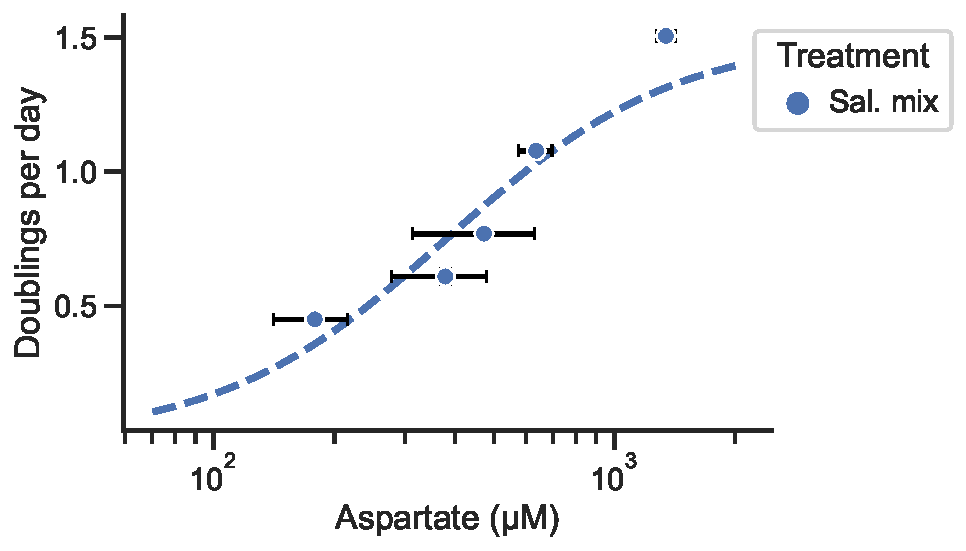
\includegraphics[width=0.49\textwidth]{figures/chap2/app/143B_Met_Asp_vs_prlfr.pdf}
    \caption[143B metformin titration aspartate to proliferation.]{
    Aspartate to proliferation relationship for 143B grown in media with salvage mix using metformin to induce aspartate limitation.
    Aspartate concentration at 50\% proliferation is 380 µM for Sal. mix treated cells.
    Salvage mix (Sal. mix) contains: 1 mM asparagine/uridine, 0.5 mM hypoxanthine, 20 µM adenine and 10 µM adenosine.
    }
    \label{fig:app_ch2:143B_Met_Asp_vs_prlfr}
\end{figure}




%\FloatBarrier
\section{tRNA charge over time}
\begin{figure}[ht]
    \centering
    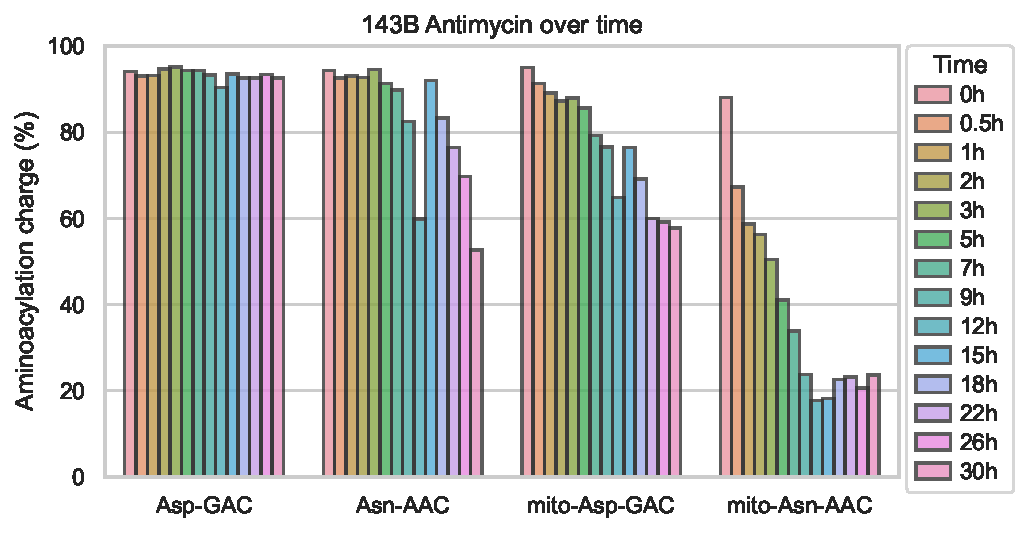
\includegraphics[width=0.7\textwidth]{figures/chap2/app/143B_Anti-time_Asp-Asn.pdf}
    \caption[Antimycin time-series in 143B, effect on tRNA charge.]{
        tRNA charge as a function of time after antimycin treatment (1 µM, spike-in) for 143B cells in DMEM, without pyruvate, with dialyzed FBS and 200 µM uridine.
    }
    \label{fig:app_ch2:143B_Anti_time}
\end{figure}




\section{Figures related to integrated stress response}
\label{sec:ch2:app:ISR}
\begin{figure}[ht]
    \centering
    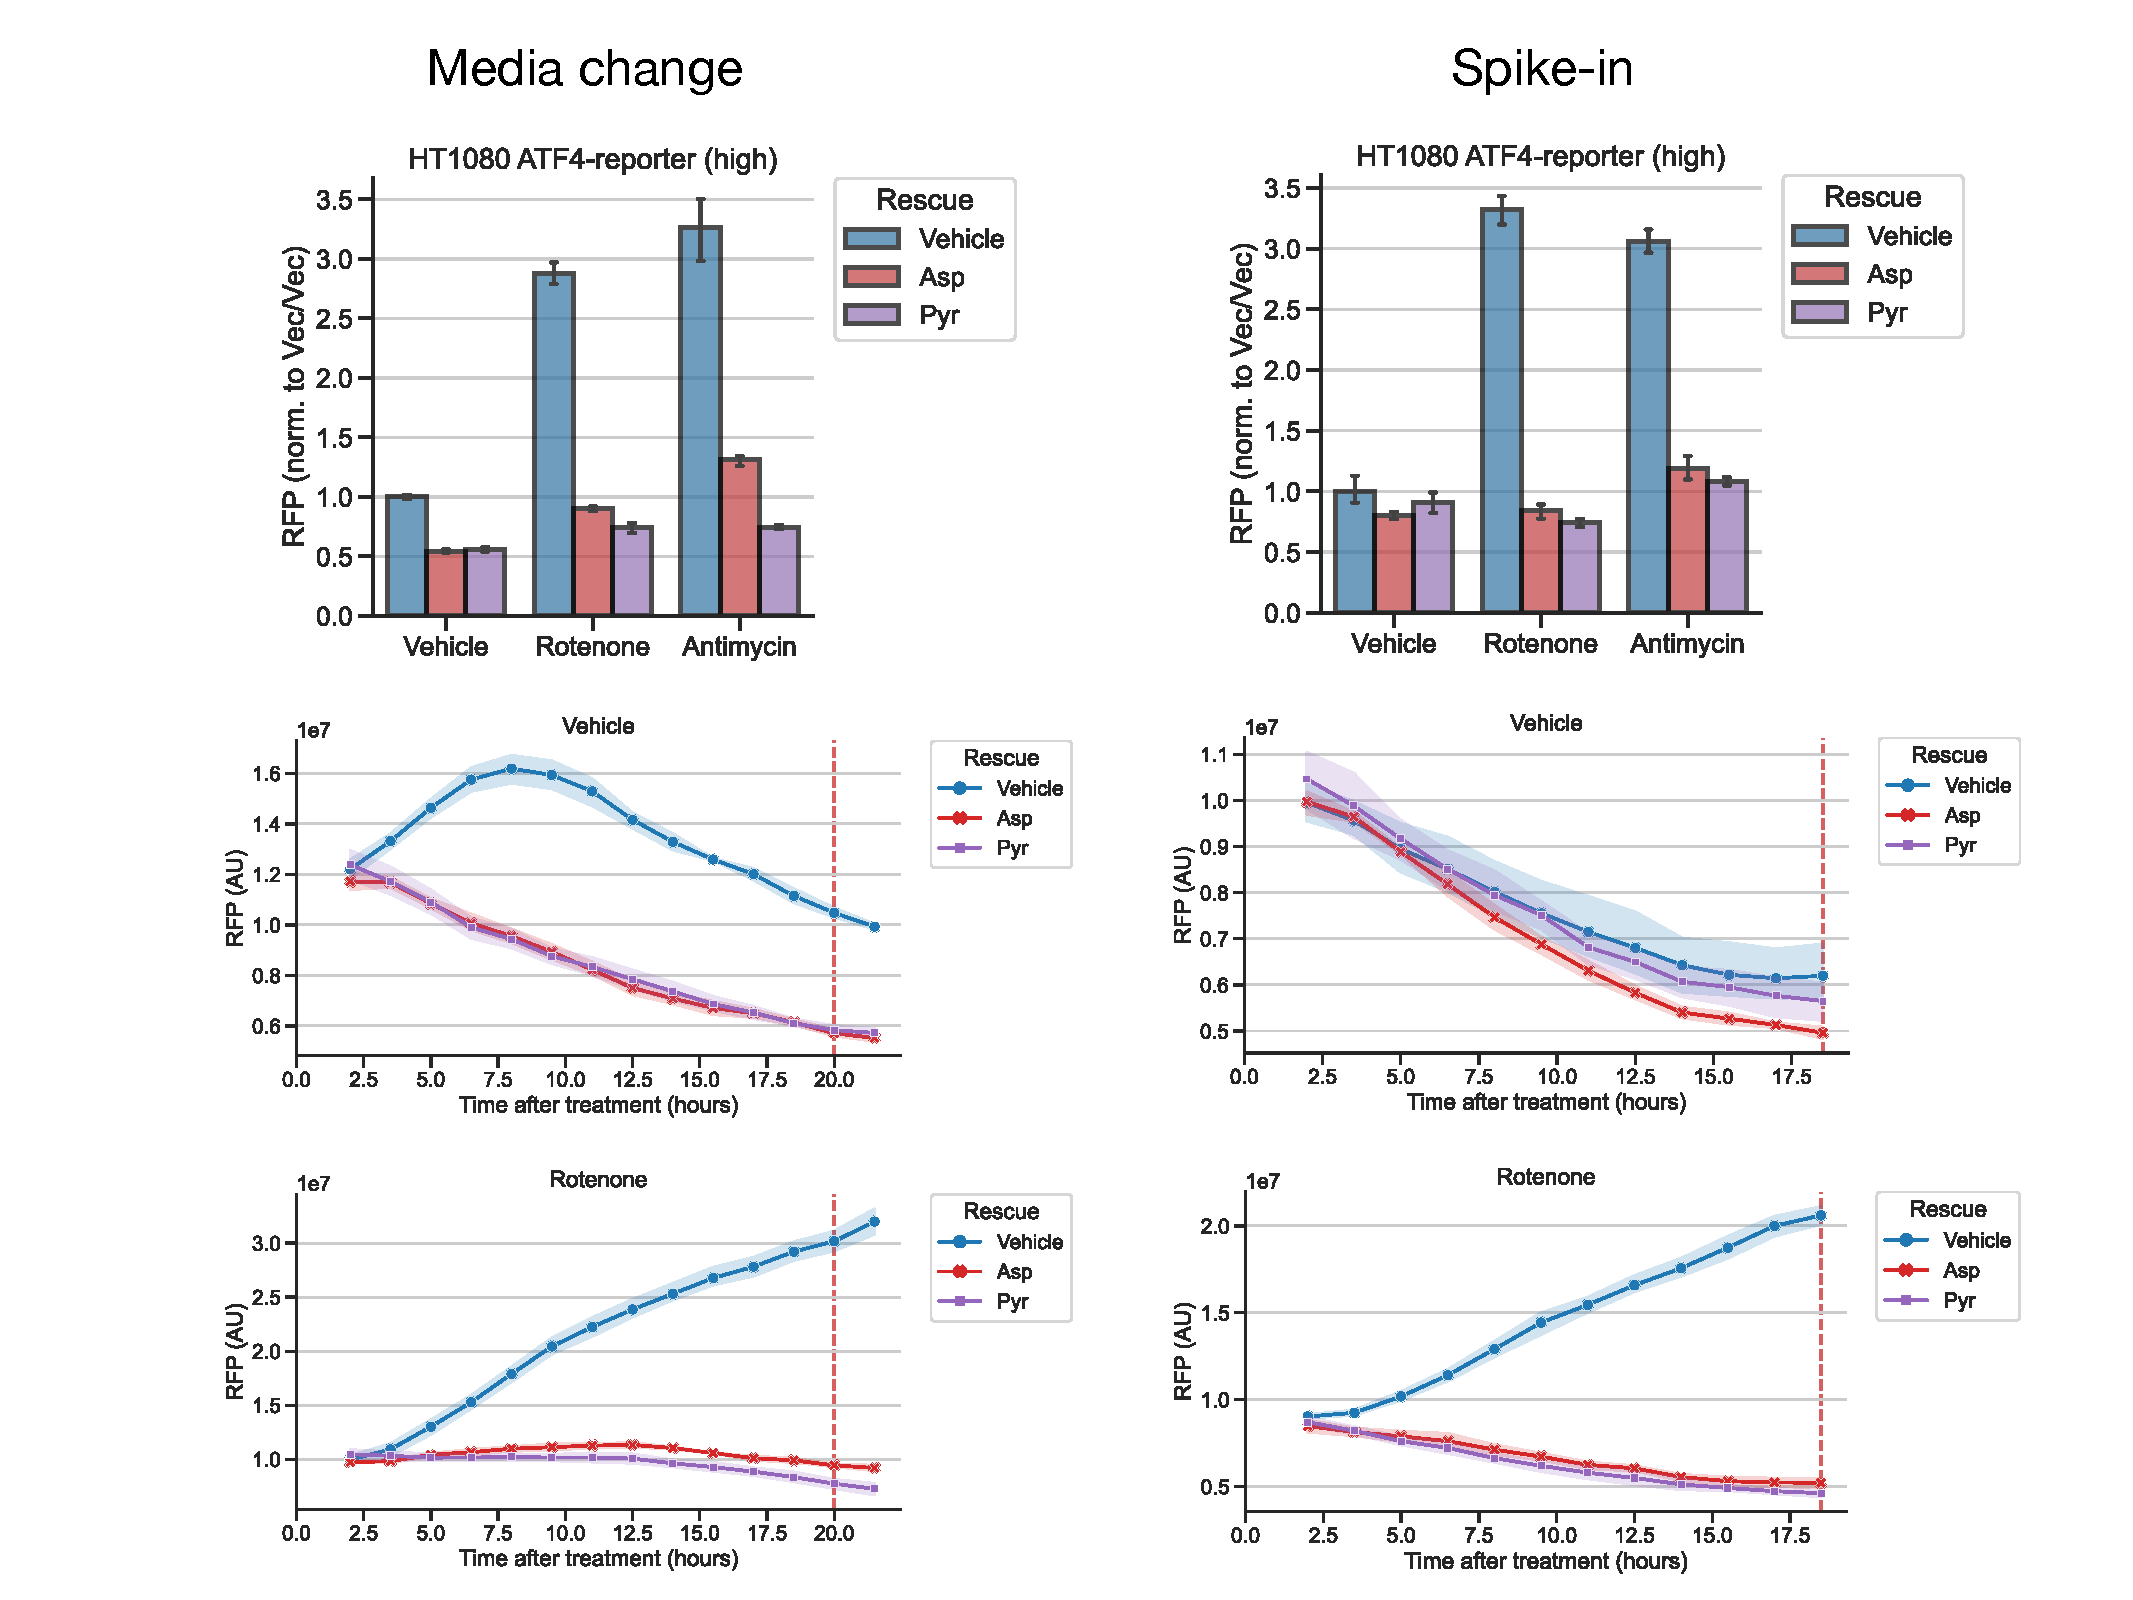
\includegraphics[width=0.95\textwidth]{figures/chap2/app/atf4_chVSsp.pdf}
    \caption[ATF4 reporter, media change vs. spike-in.]{
    Mitochondrial inhibitor induced ATF4 reporter, media change vs. spike-in.
    Left column show results from an experiment were media change was used to initiate the treatment.
    Right column show results from an experiment were the treatment was initiated by a 10x spike-in.
    Barplots show results at the time indicated by the red dashed line on the lineplots below.
    }
    \label{fig:app_ch2:atf4_chVSsp}
\end{figure}

\begin{figure}[ht]
    \centering
    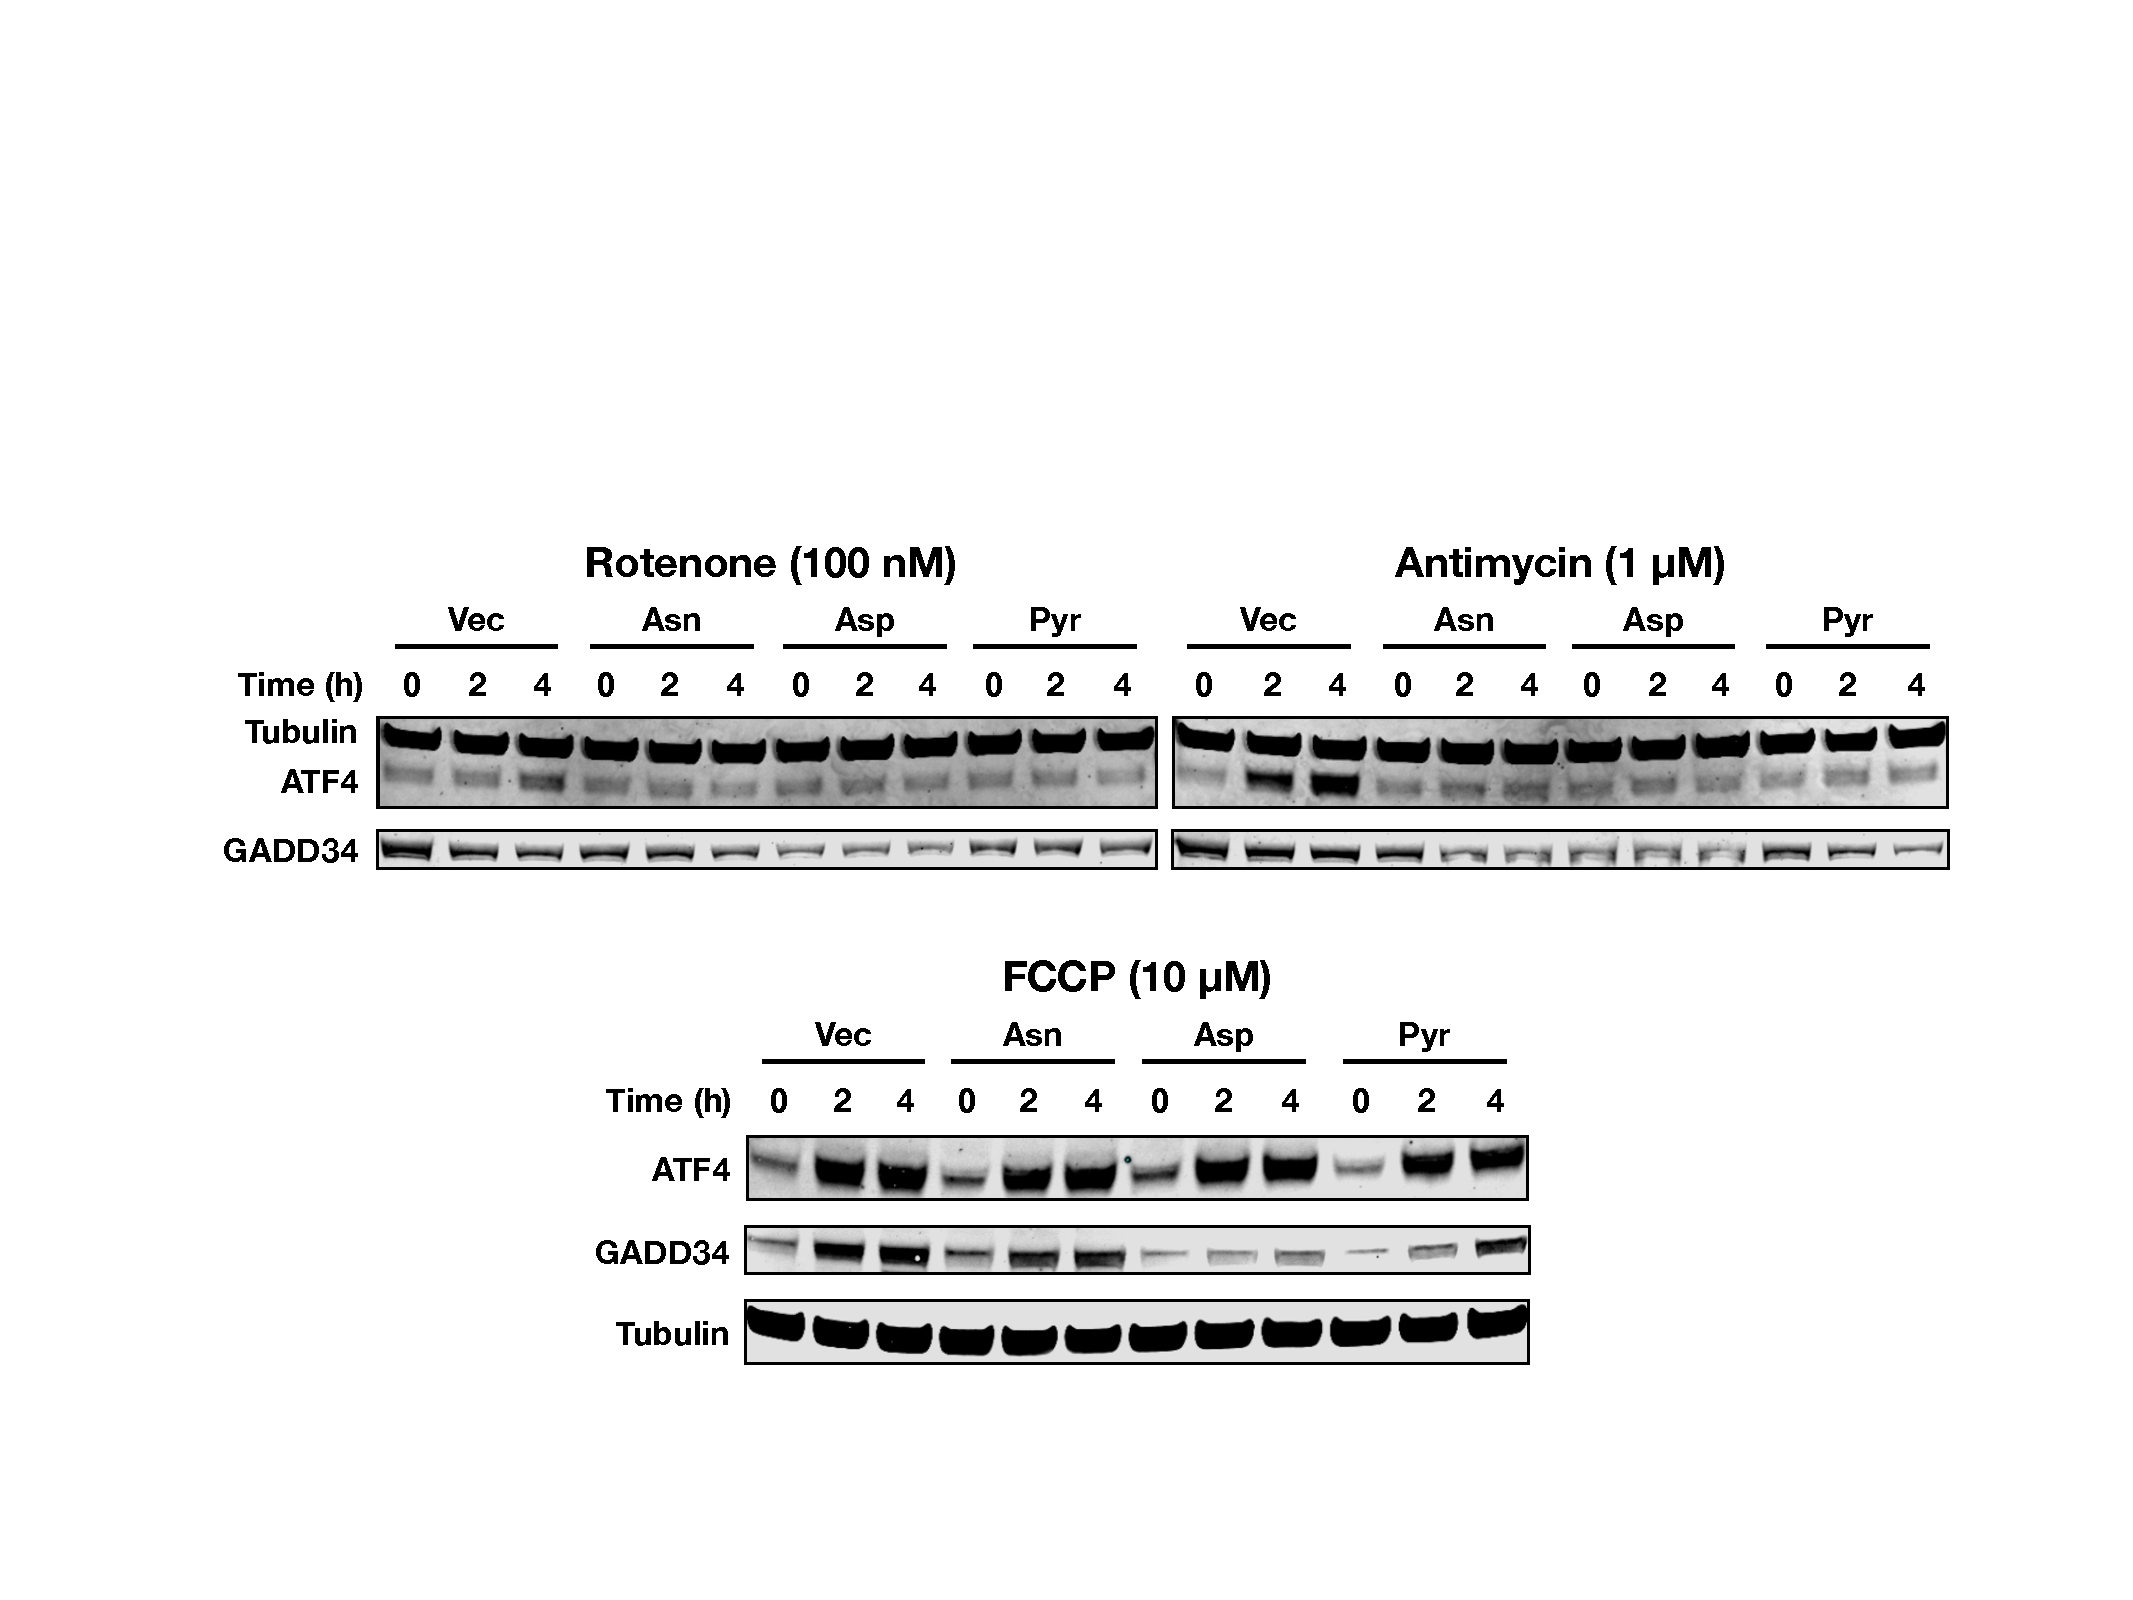
\includegraphics[width=0.95\textwidth]{figures/chap2/app/HT1080_ISR_western.pdf}
    \caption[Mitochondrial inhibitor, ATF4 western.]{
    Western blot validation of ATF4 reporter in HT1080 cells.
    Treatment and rescue conditions similar to figures \ref{fig:ch2:143B_ETCinhib_ATF4rep_low} and \ref{fig:ch2:HT1080_ETCinhib_ATF4rep_high}.
    % Wednesday 01/12/22
    }
    \label{fig:app_ch2:HT1080_ISR_western}
\end{figure}

\begin{figure}[ht]
    \centering
    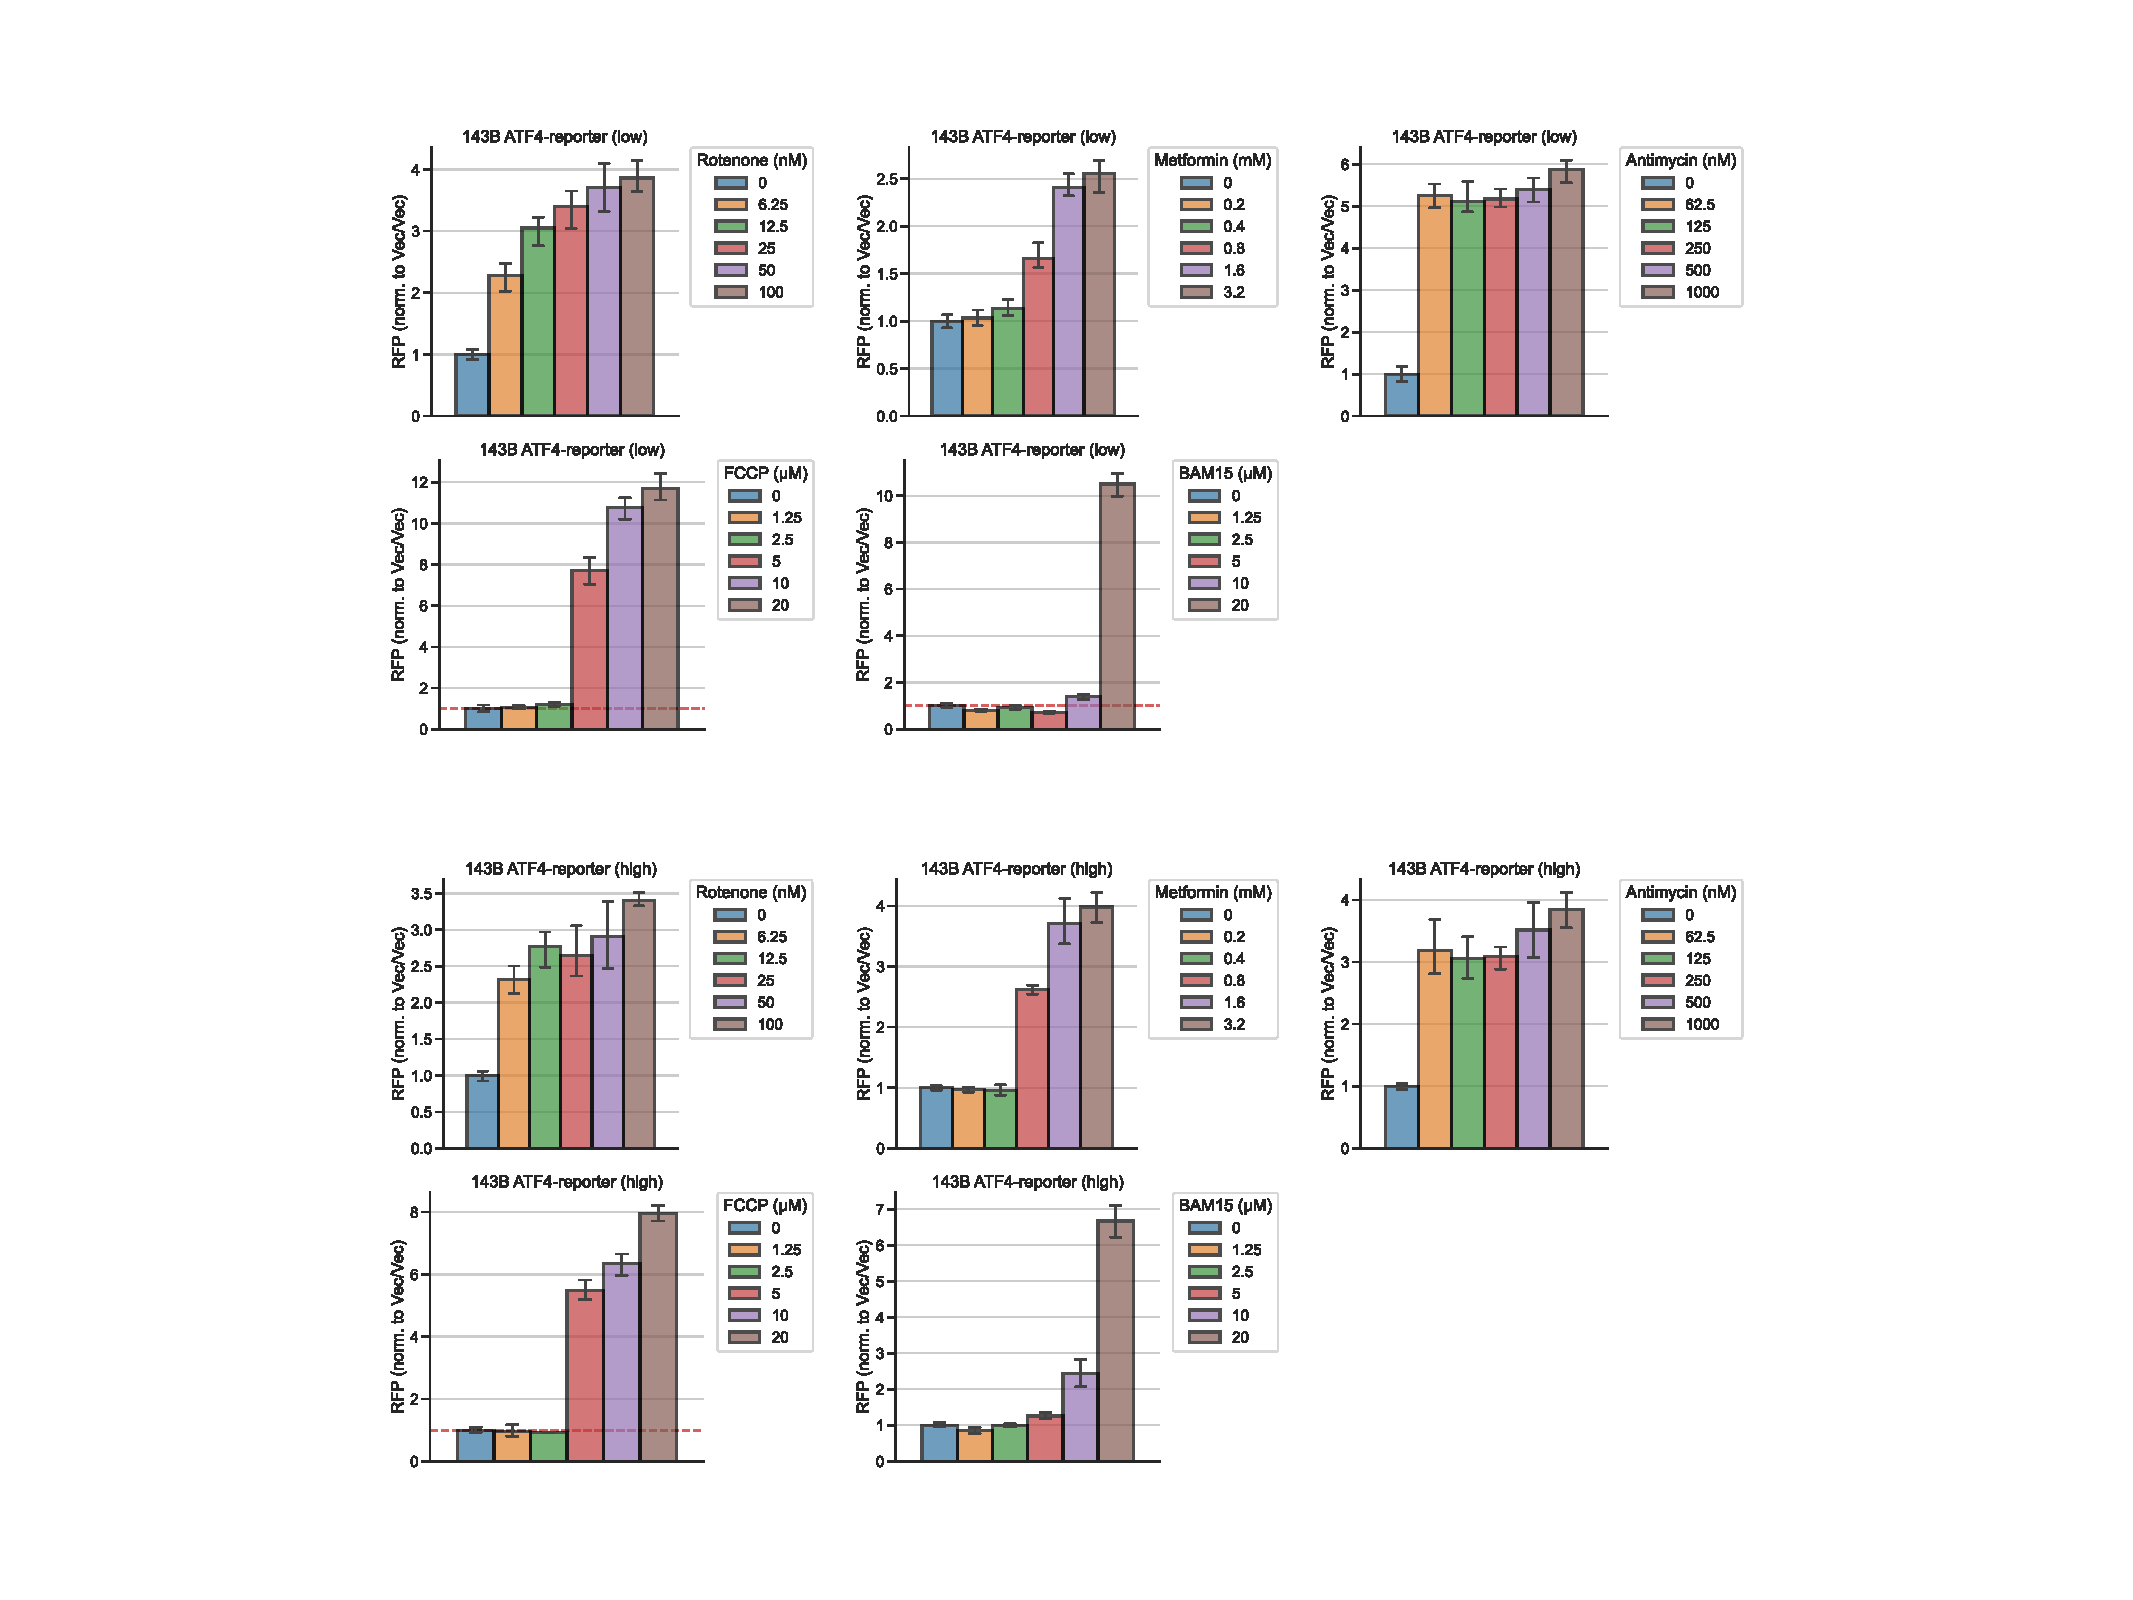
\includegraphics[width=0.95\textwidth]{figures/chap2/app/atf4_ETCtit.pdf}
    \caption[ATF4 reporter, drug titrations.]{
    ATF4 reporter, drug titrations.
    ATF4 reporter readout at 17.5 h after drug treatments of 143B cells.
    }
    \label{fig:app_ch2:atf4_ETCtit}
\end{figure}

\begin{figure}[ht]
     \centering
     \begin{subfigure}[b]{0.49\textwidth}
         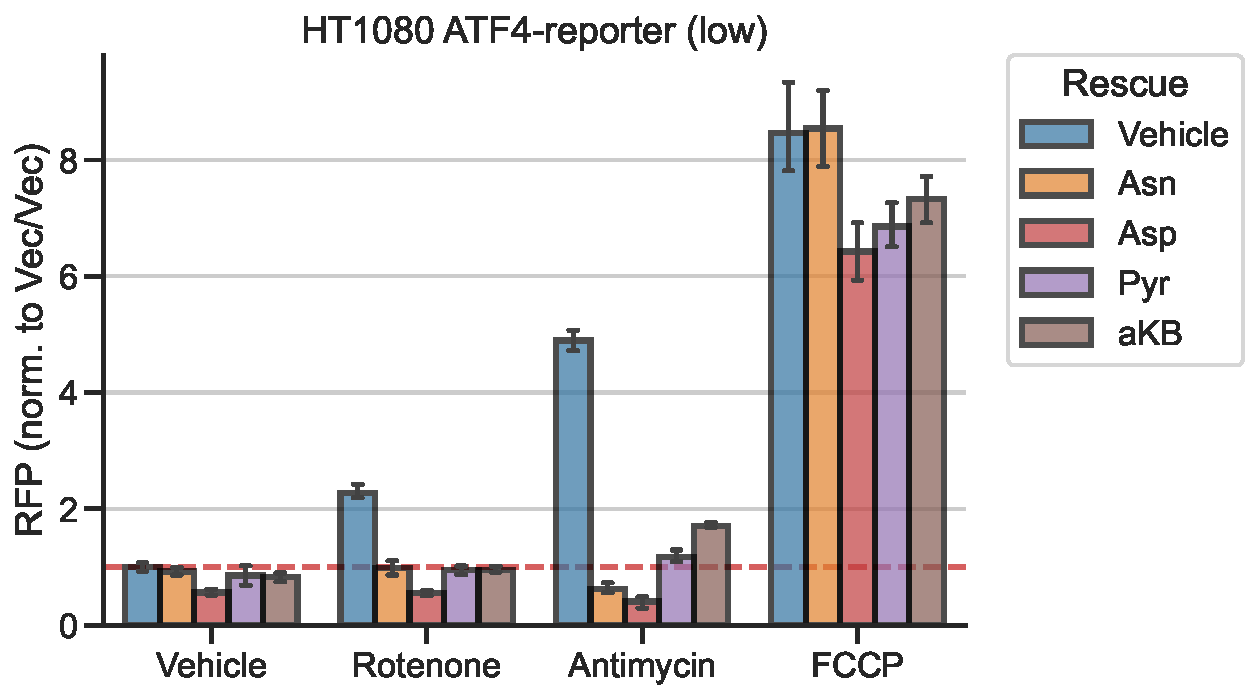
\includegraphics[width=\textwidth]{figures/chap2/app/HT1080_ETCinhib_ATF4rep_low.pdf}
         \caption{}
         \label{fig:app_ch2:HT1080_ETCinhib_ATF4rep_low}
     \end{subfigure}
     \hfill
     \begin{subfigure}[b]{0.49\textwidth}
         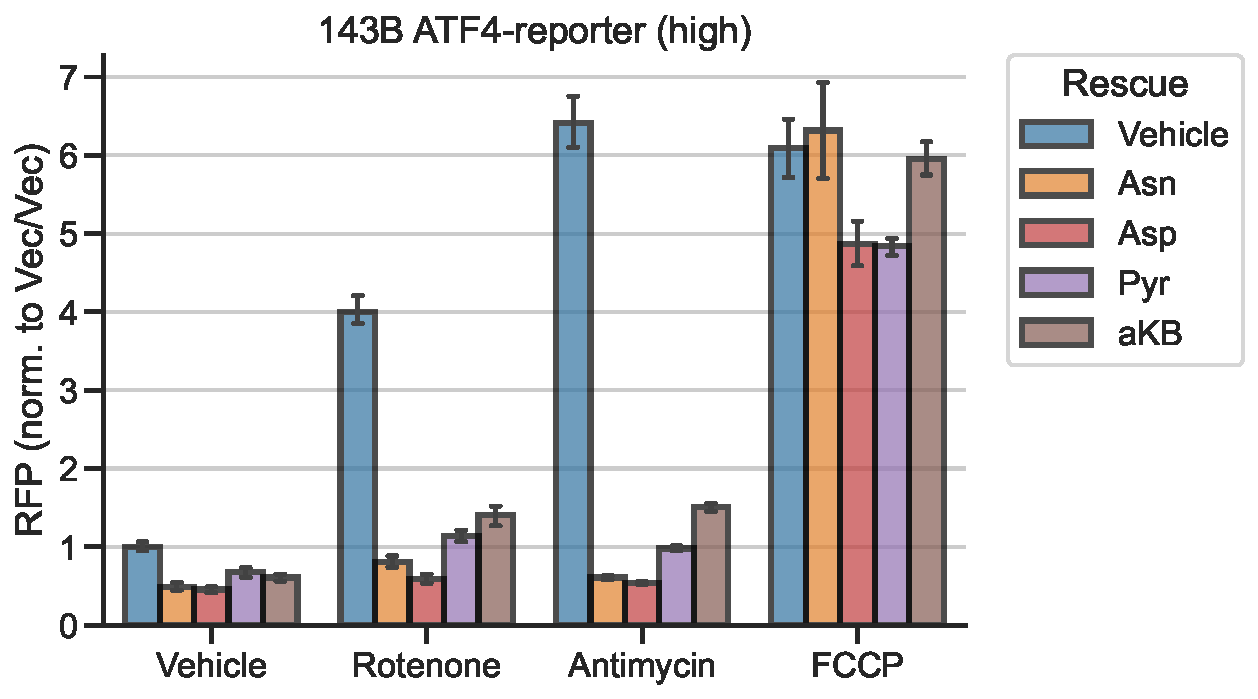
\includegraphics[width=\textwidth]{figures/chap2/app/143B_ETCinhib_ATF4rep_high.pdf}
         \caption{}
         \label{fig:app_ch2:143B_ETCinhib_ATF4rep_high}
     \end{subfigure}
     \hfill
     \begin{subfigure}[b]{0.4\textwidth}
         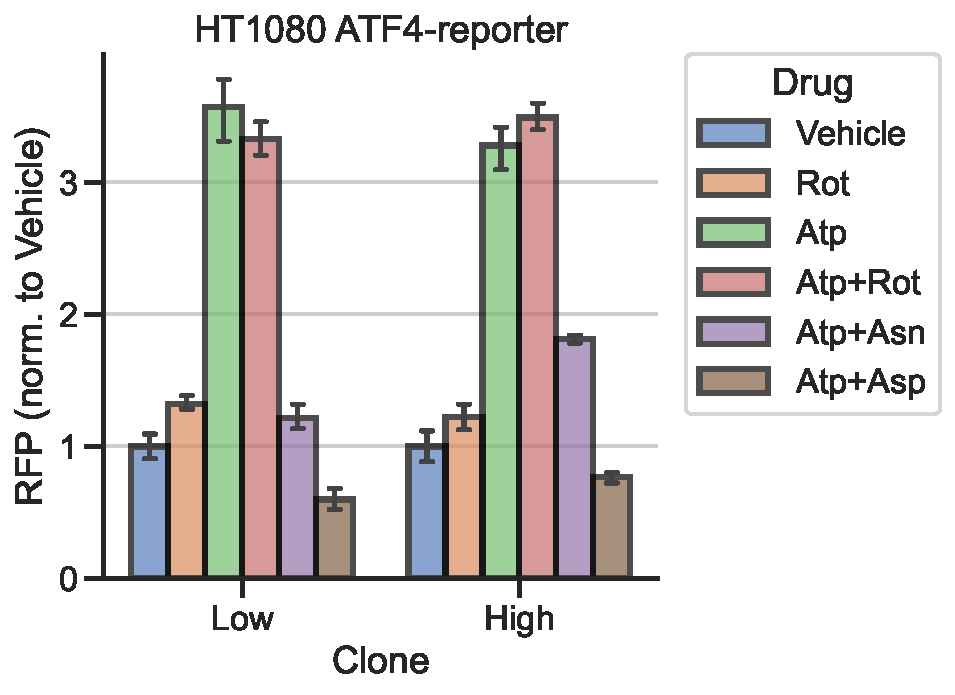
\includegraphics[width=\textwidth]{figures/chap2/app/HT1080_Atp_ATF4rep.pdf}
         \caption{}
         \label{fig:app_ch2:HT1080_Atp_ATF4rep}
     \end{subfigure}
     \hspace{0.06\textwidth}
     \begin{subfigure}[b]{0.4\textwidth}
         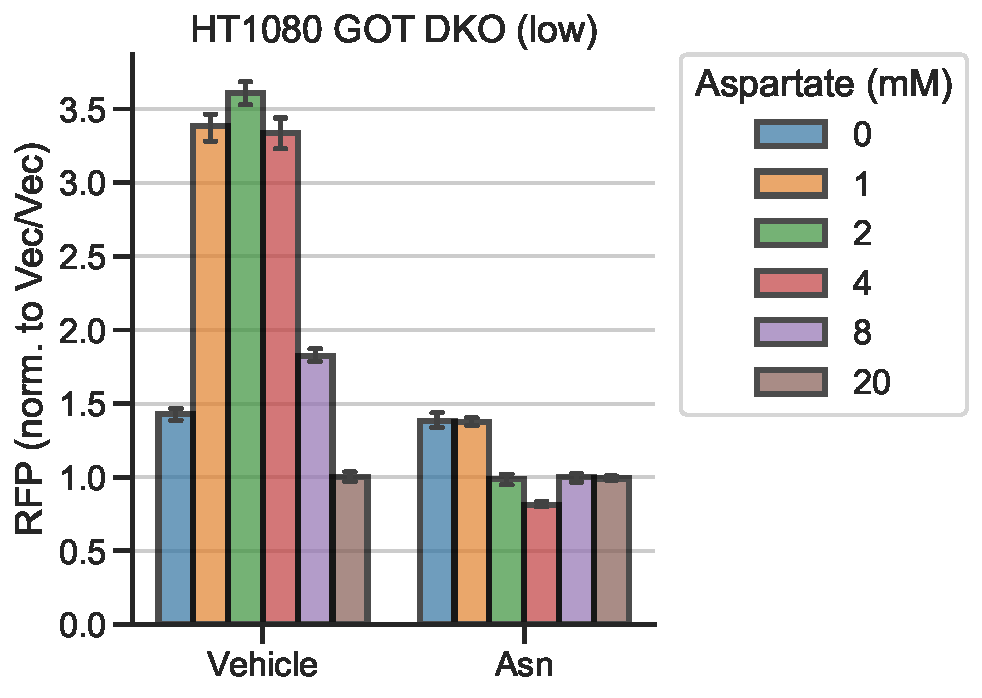
\includegraphics[width=\textwidth]{figures/chap2/app/HT1080_GOT_DKO_Asp_ATF4rep.pdf}
         \caption{}
         \label{fig:app_ch2:HT1080_GOT_DKO_Asp_ATF4rep}
     \end{subfigure}
        \caption[Mito inhibitor induced ATF4 is rescued by Asn, other clones.]{
        Panels (a), (b) and (c), related to figure \ref{fig:ch2:ISR}, here showing data generated for the other clones.
        Panel (d), GOT DKO cells respond to aspartate depletion.
        Measured 20.5 h after aspartate depletion.
        Vec/Vec normalization is normalization to the baseline condition (20 mM Asp, no Asn).
        }
        \label{fig:app_ch2:ISR}
\end{figure}

\begin{figure}[ht]
    \centering
    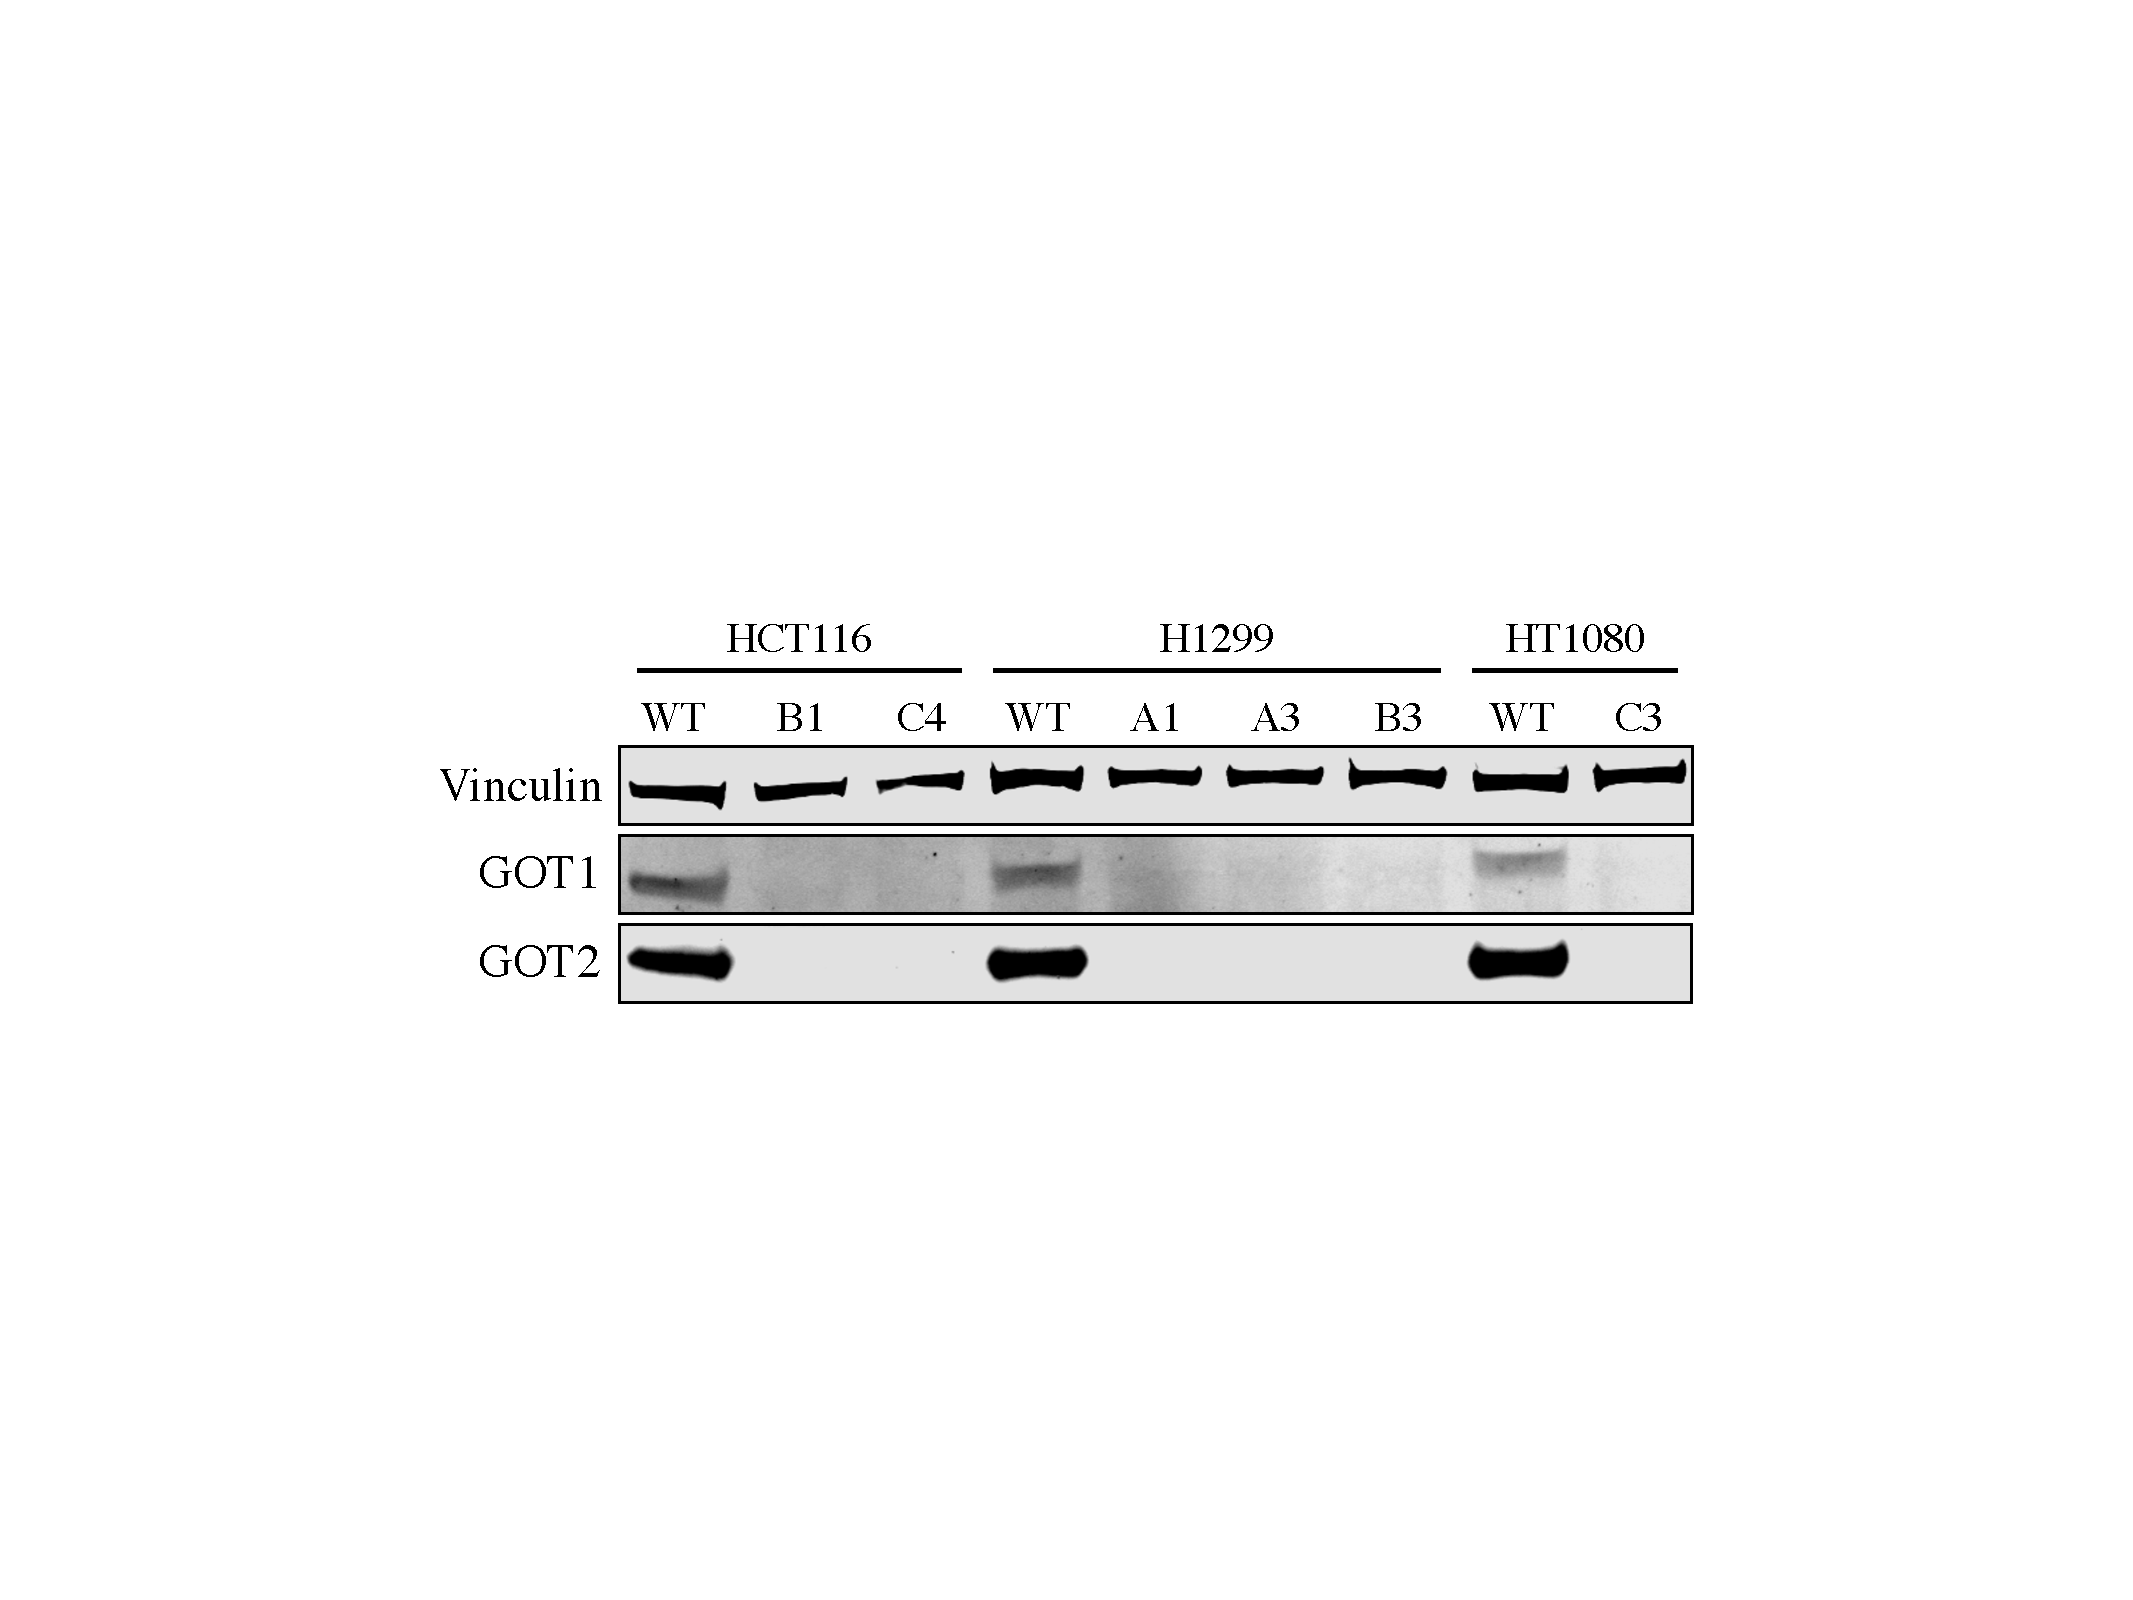
\includegraphics[width=0.55\textwidth]{figures/chap2/app/GOT_DKO_western.pdf}
    \caption[GOT DKO western blot validation.]{
    Western blot validation of GOT DKO single cell clones.
    }
    \label{fig:app_ch2:GOT_DKO_western}
\end{figure}



\newpage
\section{Antimycin induced metabolic changes}
\begin{figure}[ht!]
    \captionsetup{labelformat=empty}
    \centering
    \begin{subfigure}[b]{0.63\textwidth}
        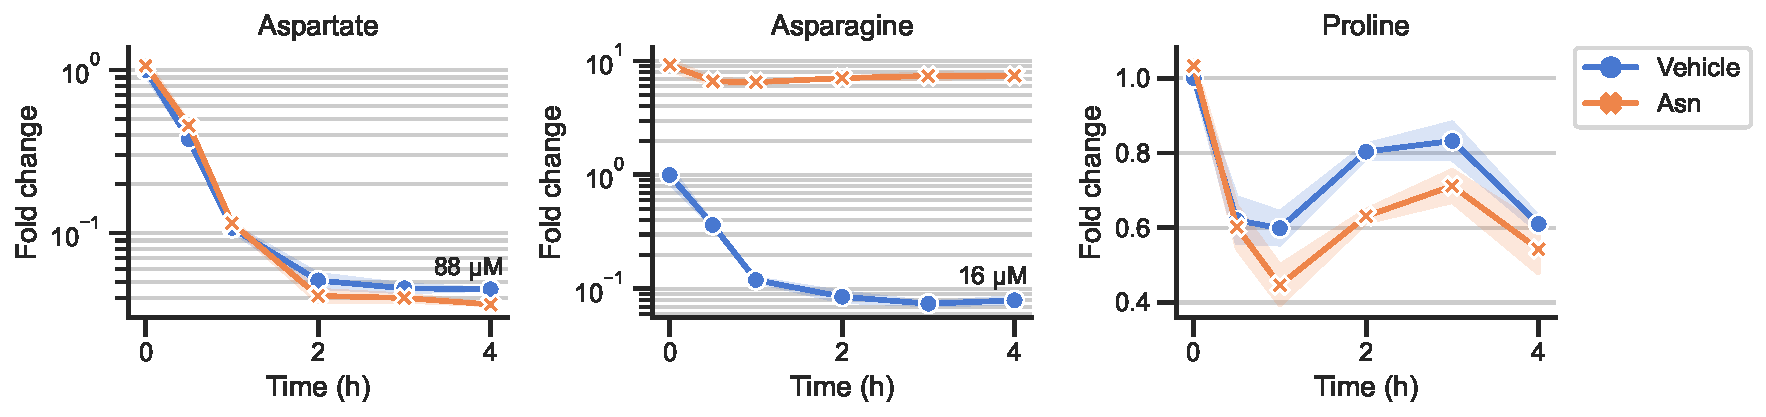
\includegraphics[width=\textwidth]{figures/chap2/app/HT1080_Anti_AA.pdf}
        \caption{Amino acids}
        \label{fig:app_ch2:HT1080_Anti_AA}
    \end{subfigure}
    \hfill
    \begin{subfigure}[b]{0.43\textwidth}
        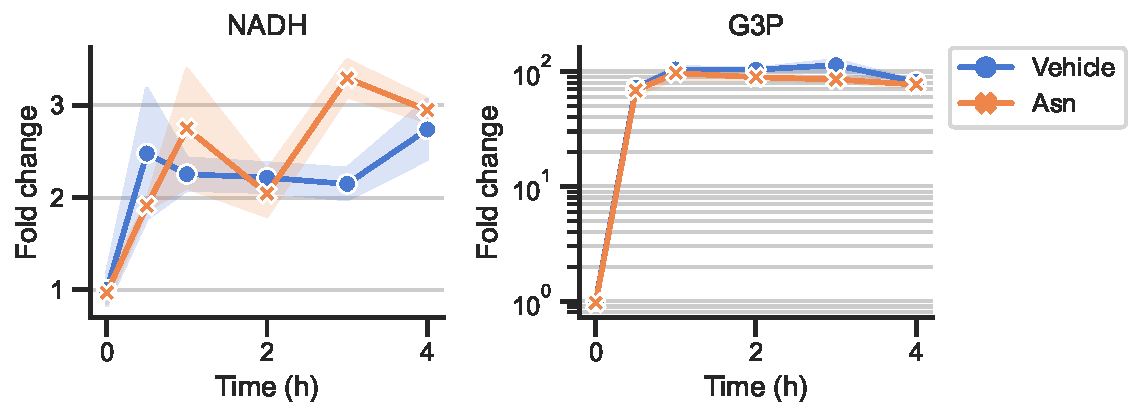
\includegraphics[width=\textwidth]{figures/chap2/app/HT1080_Anti_rd.pdf}
        \caption{Redox metabolites}
        \label{fig:app_ch2:HT1080_Anti_rd}
    \end{subfigure}
    \hfill
    \begin{subfigure}[b]{0.85\textwidth}
        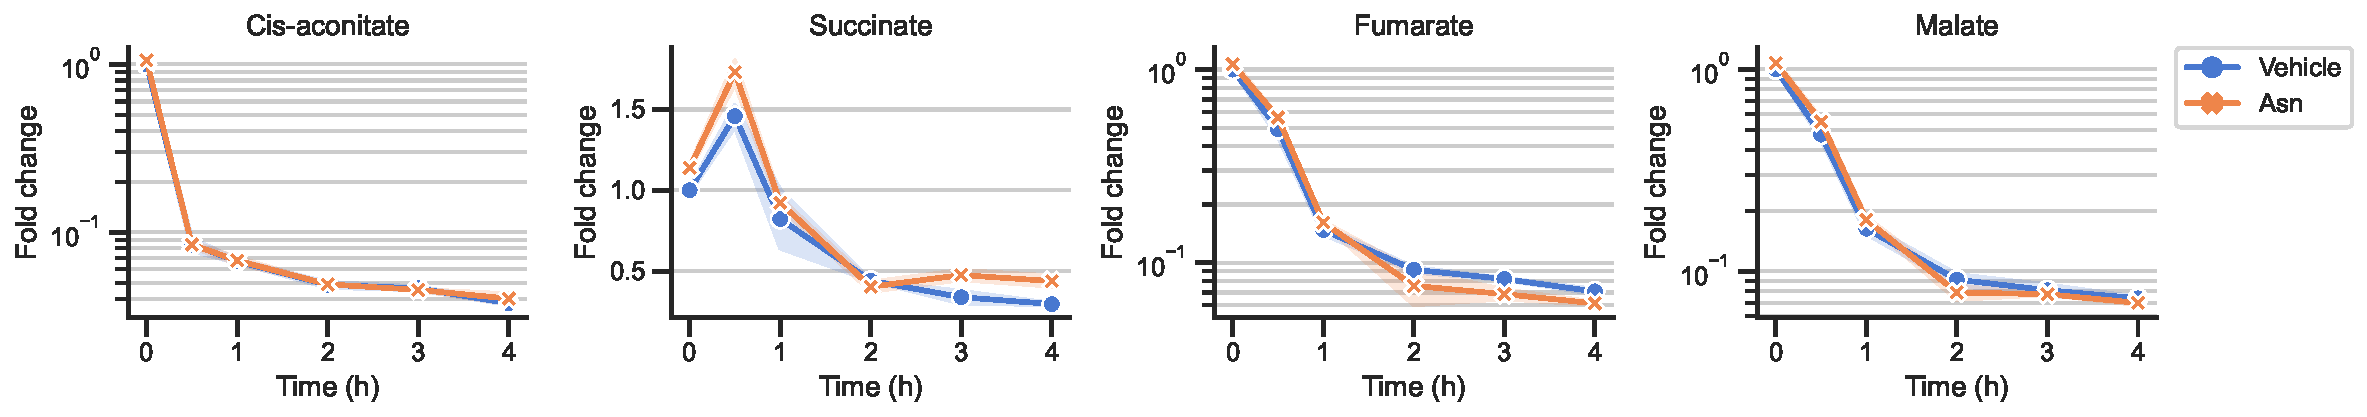
\includegraphics[width=\textwidth]{figures/chap2/app/HT1080_Anti_tca.pdf}
        \caption{TCA metabolites}
        \label{fig:app_ch2:HT1080_Anti_tca}
    \end{subfigure}
    \hfill
    \begin{subfigure}[b]{0.63\textwidth}
        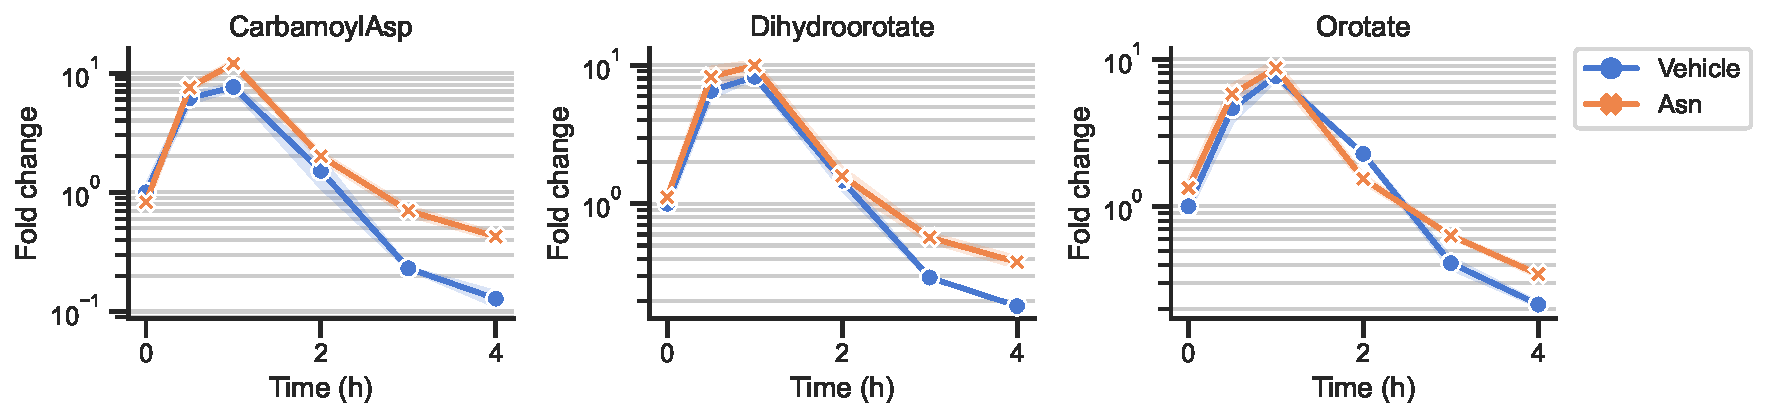
\includegraphics[width=\textwidth]{figures/chap2/app/HT1080_Anti_pyr.pdf}
        \caption{Pyrimidine metabolites}
        \label{fig:app_ch2:HT1080_Anti_pyr}
    \end{subfigure}
    \hfill
    \begin{subfigure}[b]{0.85\textwidth}
        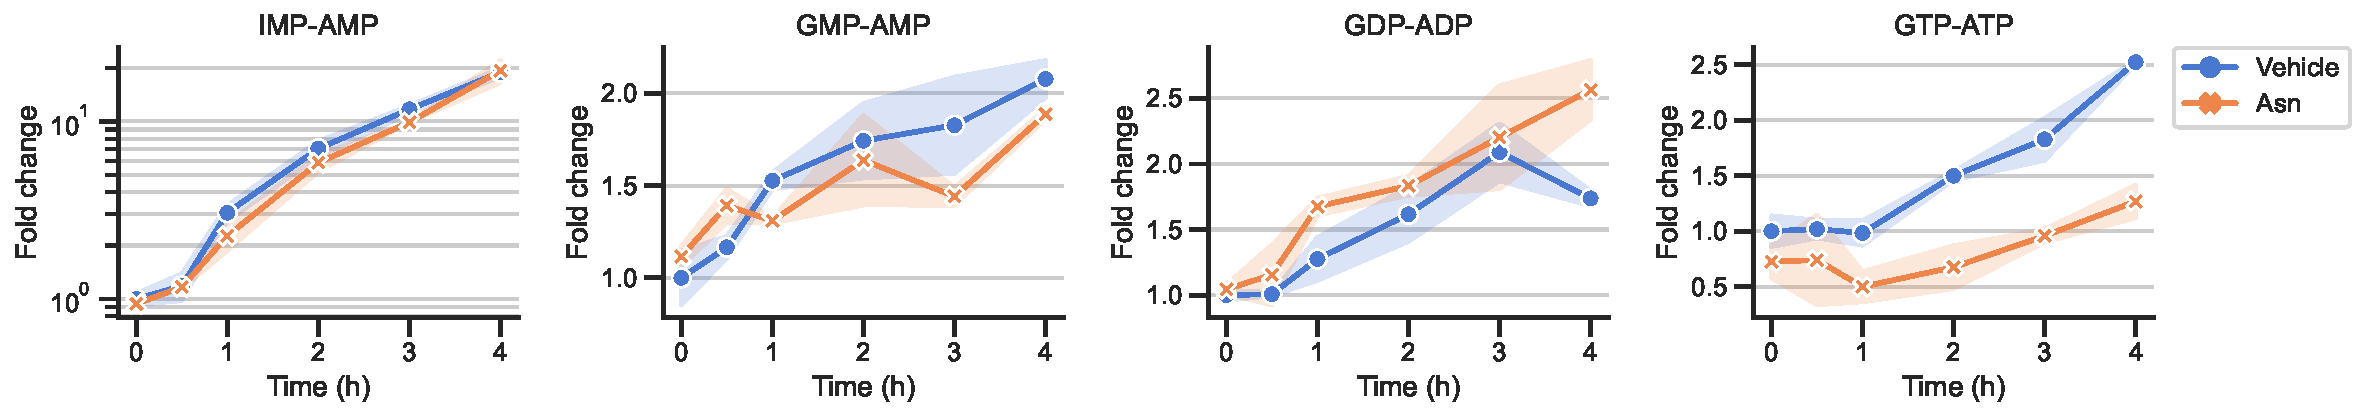
\includegraphics[width=\textwidth]{figures/chap2/app/HT1080_Anti_pur.pdf}
        \caption{Purine ratios}
        \label{fig:app_ch2:HT1080_Anti_pur}
    \end{subfigure}
    \hfill
    \caption{}
\end{figure}

\begin{figure}[ht]
    % \captionsetup{labelformat=empty}
    \ContinuedFloat
    \centering
    \begin{subfigure}[b]{0.63\textwidth}
        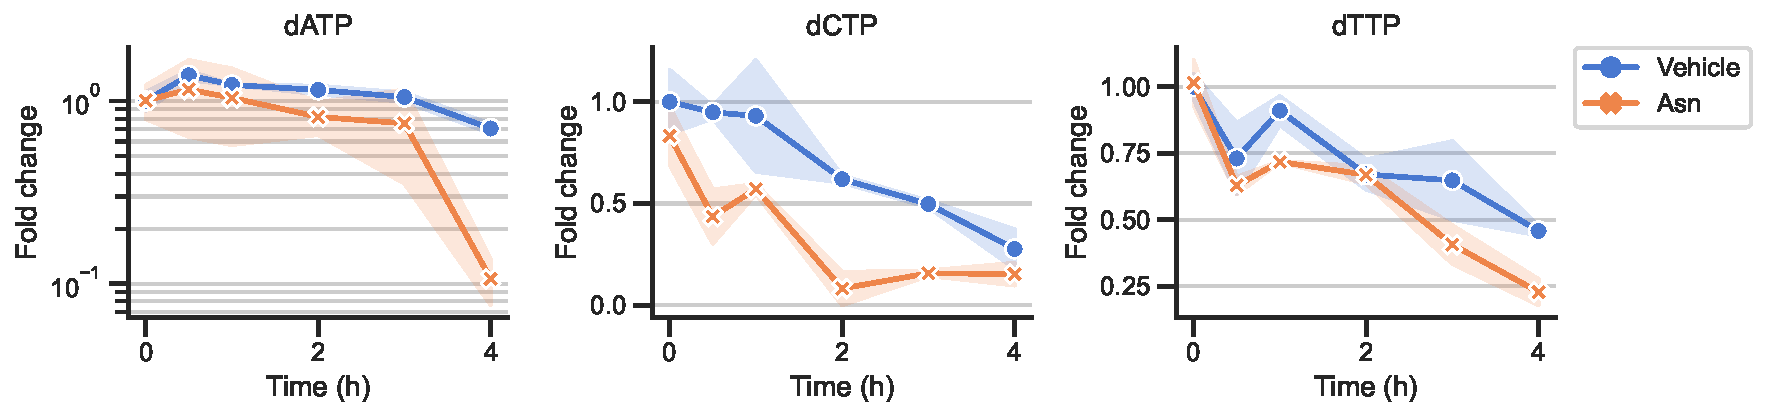
\includegraphics[width=\textwidth]{figures/chap2/app/HT1080_Anti_dntps.pdf}
        \caption{dNTPs}
        \label{fig:app_ch2:HT1080_Anti_dntps}
    \end{subfigure}
    \hfill
    \begin{subfigure}[b]{0.63\textwidth}
        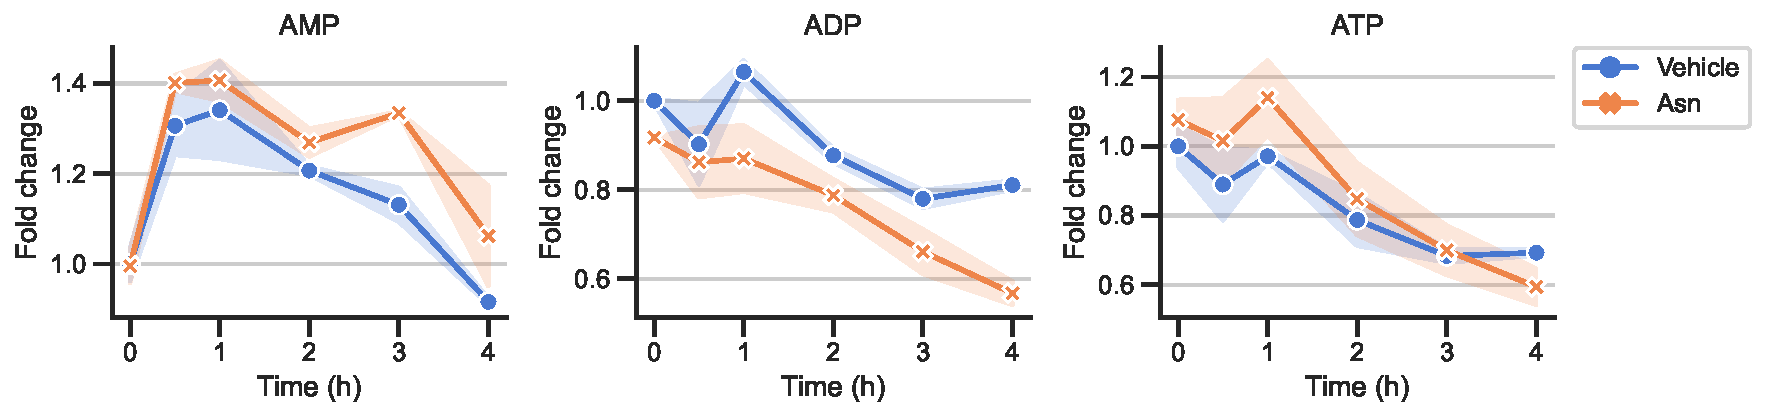
\includegraphics[width=\textwidth]{figures/chap2/app/HT1080_Anti_axp.pdf}
        \caption{AXPs}
        \label{fig:app_ch2:HT1080_Anti_axp}
    \end{subfigure}
    \hfill
    \begin{subfigure}[b]{0.63\textwidth}
        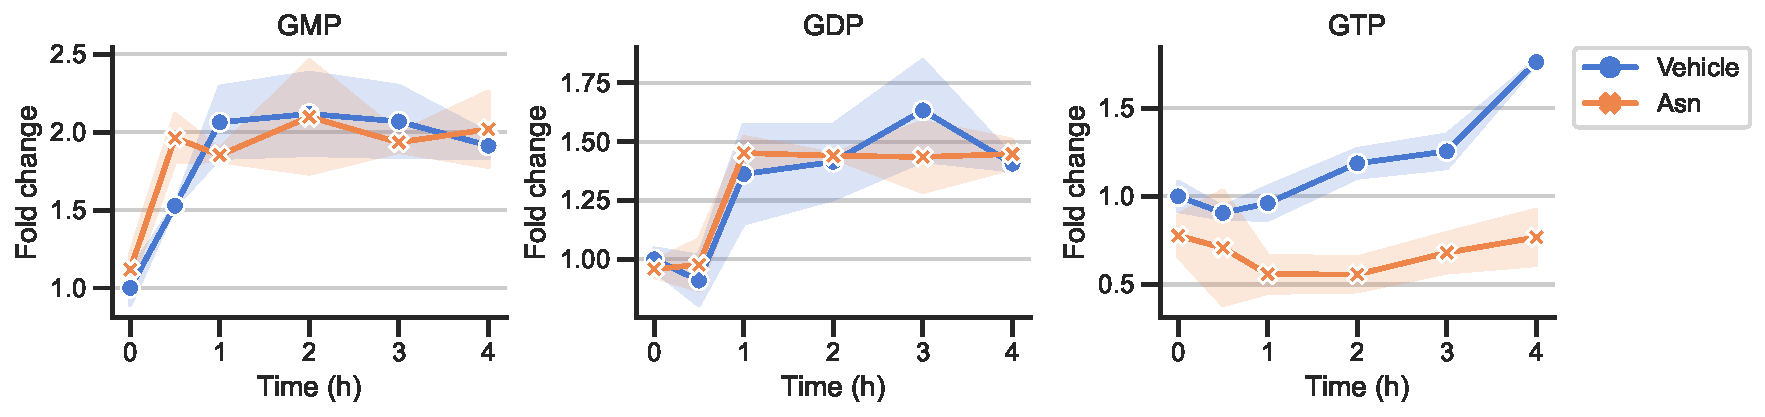
\includegraphics[width=\textwidth]{figures/chap2/app/HT1080_Anti_gxp.pdf}
        \caption{GXPs}
        \label{fig:app_ch2:HT1080_Anti_gxp}
    \end{subfigure}
    \hfill
    \begin{subfigure}[b]{0.63\textwidth}
        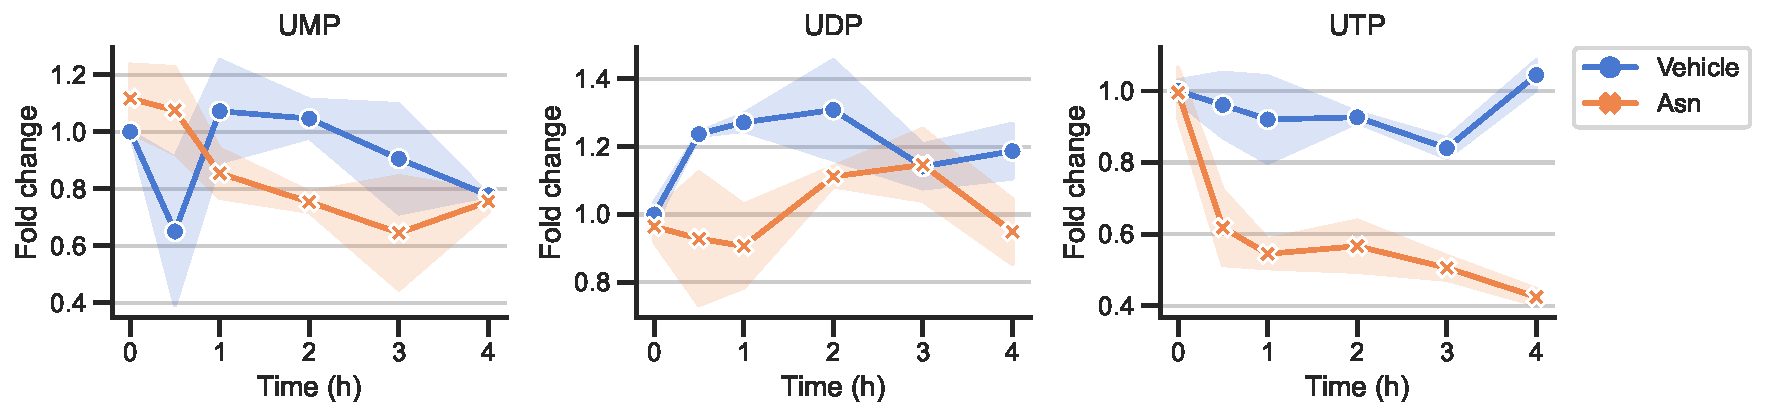
\includegraphics[width=\textwidth]{figures/chap2/app/HT1080_Anti_uxp.pdf}
        \caption{UXPs}
        \label{fig:app_ch2:HT1080_Anti_uxp}
    \end{subfigure}
    \hfill
    \begin{subfigure}[b]{0.63\textwidth}
        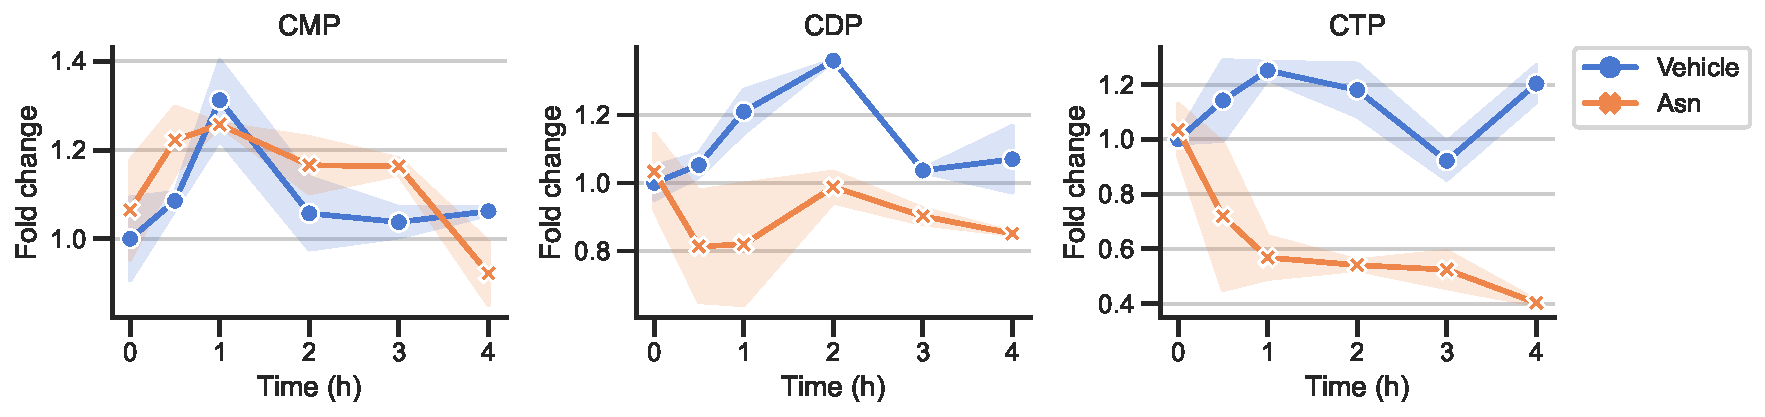
\includegraphics[width=\textwidth]{figures/chap2/app/HT1080_Anti_cxp.pdf}
        \caption{CXPs}
        \label{fig:app_ch2:HT1080_Anti_cxp}
    \end{subfigure}
    \hfill
        \caption[Metabolic changes in HT1080 after antimycin treatment.]{
        Metabolic changes in HT1080 WT after antimycin treatment (1 µM, media change).
        From same experiment as figure \ref{fig:ch2:ISR_resc}.
        }
        \label{fig:app_ch2:HT1080_Anti_metab}
\end{figure}




